%Version 3.1 December 2024
% See section 11 of the User Manual for version history
%
%%%%%%%%%%%%%%%%%%%%%%%%%%%%%%%%%%%%%%%%%%%%%%%%%%%%%%%%%%%%%%%%%%%%%%
%%                                                                 %%
%% Please do not use \input{...} to include other tex files.       %%
%% Submit your LaTeX manuscript as one .tex document.              %%
%%                                                                 %%
%% All additional figures and files should be attached             %%
%% separately and not embedded in the \TeX\ document itself.       %%
%%                                                                 %%
%%%%%%%%%%%%%%%%%%%%%%%%%%%%%%%%%%%%%%%%%%%%%%%%%%%%%%%%%%%%%%%%%%%%%

%%\documentclass[referee,sn-basic]{sn-jnl}% referee option is meant for double line spacing

%%=======================================================%%
%% to print line numbers in the margin use lineno option %%
%%=======================================================%%

%%\documentclass[lineno,pdflatex,sn-basic]{sn-jnl}% Basic Springer Nature Reference Style/Chemistry Reference Style

%%=========================================================================================%%
%% the documentclass is set to pdflatex as default. You can delete it if not appropriate.  %%
%%=========================================================================================%%

%%\documentclass[sn-basic]{sn-jnl}% Basic Springer Nature Reference Style/Chemistry Reference Style

%%Note: the following reference styles support Namedate and Numbered referencing. By default the style follows the most common style. To switch between the options you can add or remove “Numbered in the optional parenthesis. 
%%The option is available for: sn-basic.bst, sn-chicago.bst%  
 
%%\documentclass[pdflatex,sn-nature]{sn-jnl}% Style for submissions to Nature Portfolio journals
%%\documentclass[pdflatex,sn-basic]{sn-jnl}% Basic Springer Nature Reference Style/Chemistry Reference Style
\documentclass[lineno,pdflatex,sn-mathphys-num]{sn-jnl}% Math and Physical Sciences Numbered Reference Style
%%\documentclass[pdflatex,sn-mathphys-ay]{sn-jnl}% Math and Physical Sciences Author Year Reference Style
%%\documentclass[pdflatex,sn-aps]{sn-jnl}% American Physical Society (APS) Reference Style
%%\documentclass[pdflatex,sn-vancouver-num]{sn-jnl}% Vancouver Numbered Reference Style
%%\documentclass[pdflatex,sn-vancouver-ay]{sn-jnl}% Vancouver Author Year Reference Style
%%\documentclass[pdflatex,sn-apa]{sn-jnl}% APA Reference Style
%%\documentclass[pdflatex,sn-chicago]{sn-jnl}% Chicago-based Humanities Reference Style

%%%% Standard Packages
%%<additional latex packages if required can be included here>

\usepackage{graphicx}%
\usepackage{multirow}%
\usepackage{amsmath,amssymb,amsfonts}%
\usepackage{amsthm}%
\usepackage{mathrsfs}%
\usepackage[title]{appendix}%
\usepackage{xcolor}%
\usepackage{textcomp}%
\usepackage{manyfoot}%
\usepackage{booktabs}%
\usepackage{algorithm}%
\usepackage{algorithmicx}%
\usepackage{algpseudocode}%
\usepackage{listings}%
%%%%

%%%%%=============================================================================%%%%
%%%%  Remarks: This template is provided to aid authors with the preparation
%%%%  of original research articles intended for submission to journals published 
%%%%  by Springer Nature. The guidance has been prepared in partnership with 
%%%%  production teams to conform to Springer Nature technical requirements. 
%%%%  Editorial and presentation requirements differ among journal portfolios and 
%%%%  research disciplines. You may find sections in this template are irrelevant 
%%%%  to your work and are empowered to omit any such section if allowed by the 
%%%%  journal you intend to submit to. The submission guidelines and policies 
%%%%  of the journal take precedence. A detailed User Manual is available in the 
%%%%  template package for technical guidance.
%%%%%=============================================================================%%%%

%% as per the requirement new theorem styles can be included as shown below
\theoremstyle{thmstyleone}%
\newtheorem{theorem}{Theorem}%  meant for continuous numbers
%%\newtheorem{theorem}{Theorem}[section]% meant for sectionwise numbers
%% optional argument [theorem] produces theorem numbering sequence instead of independent numbers for Proposition
\newtheorem{proposition}[theorem]{Proposition}% 
%%\newtheorem{proposition}{Proposition}% to get separate numbers for theorem and proposition etc.

\theoremstyle{thmstyletwo}%
\newtheorem{example}{Example}%
\newtheorem{remark}{Remark}%

\theoremstyle{thmstylethree}%
\newtheorem{definition}{Definition}%

\raggedbottom
%%\unnumbered% uncomment this for unnumbered level heads

\usepackage{amsmath}    % for \text{} inside equations
\usepackage{multirow}   % optional, for merged table cells
\usepackage{tikz}
\usepackage{url}
\usetikzlibrary{arrows.meta,positioning}
\usetikzlibrary{calc}
\usetikzlibrary{patterns}
\usepackage{pgfplots}   % bar charts

\begin{document}

\title[Article Title]{Where Do Vision Foundation Models Look? A Comparative Study of Attention Alignment in Architectural Image Recognition}

%%=============================================================%%
%% GivenName	-> \fnm{Joergen W.}
%% Particle	-> \spfx{van der} -> surname prefix
%% FamilyName	-> \sur{Ploeg}
%% Suffix	-> \sfx{IV}
%% \author*[1,2]{\fnm{Joergen W.} \spfx{van der} \sur{Ploeg} 
%%  \sfx{IV}}\email{iauthor@gmail.com}
%%=============================================================%%

\author[1]{\fnm{First} \sur{Author}}\email{first author@u.nus.edu}
\author[1]{\fnm{Second} \sur{Author}}\email{second author@u.nus.edu}
\author*[1]{\fnm{Jing} \sur{Tian}}\email{tianjing@nus.edu.sg}
\author[1]{\fnm{Xavier Zhen} \sur{Xie}}\email{xav.xie@nus.edu.sg}

\affil*[1]{\orgdiv{NUS-ISS}, \orgname{National University of Singapore}, \orgaddress{\street{25 Heng Mui Keng Ter}, \city{Singapore}, \postcode{119615}, \country{Singapore}}}


%%==================================%%
%% Sample for unstructured abstract %%
%%==================================%%

\abstract{Self-supervised vision foundation models achieve strong downstream performance, but high
classification accuracy alone does not reveal whether those models attend to the
same visual evidence that human experts consider diagnostically important. This
project studies that question in the WikiChurches setting, where expert bounding
boxes identify architectural features such as arches, windows, towers, and
facade elements that matter for style recognition.

We evaluate seven vision foundation models across self-distillation, masked autoencoding,
multimodal contrastive pretraining, and a supervised CNN baseline, then measure
attention alignment against 631 expert boxes on 139 annotated church images
using IoU, Coverage, MSE, KL divergence, and EMD.

The study is organised around three linked questions:
(1)~How well frozen models align with expert-marked regions;
(2)~How Linear Probe, LoRA, and Full fine-tuning change that alignment;
(3)~Whether individual attention heads exhibit descriptive specialisation for
different architectural features.

}


\keywords{Explainable computer vision, vision foundation model, self-supervised learning, attention map, architectural recognition}

%%\pacs[JEL Classification]{D8, H51}

%%\pacs[MSC Classification]{35A01, 65L10, 65L12, 65L20, 65L70}

\maketitle

\clearpage

\section{Introduction}

\cite{Hasic26NN, Remi25IF, Wan26PAMI, Kashefi2026review}

grad-cam \cite{Selvaraju17GradCAM}, Deep Taylor Decomposition \cite{Chefer21Interp}

A vision model can be correct for the wrong visual reasons. In architectural
style recognition, a model that classifies a church as Gothic because it attends
to pointed arches and flying buttresses is qualitatively different from one that
succeeds because it exploits background regularities or photographer bias
unrelated to expert reasoning. Accuracy alone cannot distinguish those cases.

WikiChurches~\cite{Barz21WikiChurches} provides a strong evaluation setting
because it pairs fine-grained architectural-style labels with expert bounding
boxes marking characteristic visual features, making it possible to compare
model attention directly against human expert targets rather than inferring
plausibility from class predictions alone.

This report addresses three linked research questions. \textbf{Q1}: Do frozen
SSL and baseline vision foundation models attend to the same architectural regions that
experts mark as diagnostically important?  \textbf{Q2}: Do individual attention heads exhibit descriptive specialisation for different architectural features, and do dominant heads shift
across variants? \textbf{Q3}: How does attention change
after adaptation (Linear Probe, LoRA, Full fine-tuning), and does strategy
matter?

Taken together, these questions shift the project from a visualisation exercise
into a domain-grounded evaluation study of what different pretraining and
adaptation choices encourage models to attend to.



% \begin{table}[!h]
% \begin{tabular}{ccccccccc}
% \hline
% Method & \multicolumn{2}{c}{Research focus} & Dataset & \multicolumn{2}{c}{Model} & \multicolumn{2}{c}{Model's output}  & Finetuing \\
%  & Explanation & Evaluation &  & supervised & self-supervised & intermediate & final &  \\ \hline
% \cite{Kang20259339} & $\checkmark$ & $-$ & General & $-$ & $\checkmark$ & $\checkmark$ & $-$ & $-$ \\
% \cite{Jo2025582} & $\checkmark$ & $-$ & General & $\checkmark$ & $-$ & $\checkmark$ & $\checkmark$ & $-$ \\
% \cite{Liao2025PR} & $\checkmark$ & $-$ & General & $\checkmark$ & $\checkmark$ & $\checkmark$ & $\checkmark$ & $-$ \\
% \cite{Hanna25ICCV} & $\checkmark$ & $-$ & General, medical, & $\checkmark$ & $-$ & $-$ & $\checkmark$ & $-$ \\
%  &  &  & remote sensing &  &  &  &  & \\
% \cite{Cascone25ICCV} & $\checkmark$ & $-$ & Medical & $\checkmark$ & $-$ & $-$ & $\checkmark$ & $-$ \\
% \cite{Hasannezhad2025} & $\checkmark$ & $-$ & Medical & $\checkmark$ & $-$ & $-$ & $\checkmark$ & $-$ \\
% \cite{Velvizhi2026} & $\checkmark$ & $-$ & Medical & $\checkmark$ & $-$ & $-$ & $\checkmark$ & $-$ \\
% \cite{park2023what} & $-$ & $\checkmark$ & General & $-$ & $\checkmark$ & $\checkmark$ & $\checkmark$ & $-$ \\
% \cite{Walmer23CVPR} & $-$ & $\checkmark$ & General & $\checkmark$ & $-$ & $\checkmark$ & $\checkmark$ & $\checkmark$ \\
% \cite{Carrasco2026} & $-$ & $\checkmark$ & Image stimuli & $\checkmark$ & $-$ & $\checkmark$ & $\checkmark$ & $-$ \\
%  &  &  & and eye tracking &  &  &  &  & \\
% \cite{Yamamoto2025} & $-$ & $\checkmark$ & Image stimuli & $\checkmark$ & $-$ & $\checkmark$ & $\checkmark$ & $-$ \\
%  &  &  & and human gaze &  &  &  &  & \\
% \cite{Cascone2026947} & $-$ & $\checkmark$ & Medical & $\checkmark$ & $-$ & $\checkmark$ & $\checkmark$ & $-$ \\
% \cite{Chung2025110} & $-$ & $\checkmark$ & Medical & $\checkmark$ & $-$ & $-$ & $\checkmark$ & $\checkmark$ \\ \hline
% Ours & $-$ & $\checkmark$ & Architectual image & $-$ & $\checkmark$ & $\checkmark$ & $\checkmark$ & $\checkmark$ \\ \hline
% \end{tabular}
% \end{table}

\section{Related Work} \label{section related works}

\subsection{Explaining vision foundation models}

Many studies have shown how attention maps and activation-based visualizations can be used to explain the behavior of vision foundation models. These attention-based methods leverage the native self-attention structure of ViTs. The raw attention visualization derived from the final transformer layers serves as a baseline inspection tool in the original ViT formulation \cite{dosovitskiy21vit}. Furthermore, attention signals become progressively entangled across layers inside the ViT model \cite{Abnar20Rollout}.

For ViT interpretability, several methods refine the use of attention maps beyond simple averaging or raw visualization. Kang et al.~\cite{Kang20259339} investigate whether frozen large vision-language models contain attention heads that already encode object localization behavior. Rather than adding task-specific grounding heads or fine-tuning the model, their method identifies a small subset of localization heads and uses text-to-image attention maps to recover image regions associated with textual descriptions.  A gradient-driven multi-head attention rollout is proposed to estimate the relative importance of individual attention heads using gradient-derived scores and then aggregates head-level attention with learned weights \cite{Jo2025582}. This addresses the limitation that not all heads contribute equally to a model decision. A dynamic accumulated attention map is proposed to focuse on the temporal evolution of attention across transformer blocks \cite{Liao2025PR}. By decomposing class-token representations and accumulating block-wise attention information, it emphasizes layer-wise attention flow and the formation of decision evidence inside the transformer.


Other works adapt attention-based explanations to weakly supervised or domain-specific prediction tasks. Hanna et al.~\cite{Hanna25ICCV} propose a sparse ViT with multiple class-specific \texttt{[CLS]} tokens for weakly supervised semantic segmentation. Their method encourages each class token to specialize through masking and then uses the corresponding self-attention maps to generate pseudo-segmentation masks. This differs from post-hoc explanation approaches because the model architecture and training procedure are designed to make class-specific attention more directly usable as an explanation. In medical imaging, Cascone et al.~\cite{Cascone25ICCV} build an interpretable diabetic retinopathy grading framework, using the transformer backbone as both a representation learner and a source of explanation for clinical decision support. Hasannezhad et al.~\cite{Hasannezhad2025} develop a transformer-based UNet for medical image segmentation, using class activation maps to enhance local features before transformer-based global modeling. Velvizhi et al.~\cite{Velvizhi2026} develop an explainable ViT for stenosis diagnosis in X-ray coronary angiography, by localizing discriminative regions without relying on gradients. 

\subsection{Measuring and benchmarking model explanations}

The other related work evaluates what attention maps and visual explanations actually capture. 

The first category of works measures how training objectives influence internal attention mechanisms. Park et al.~\cite{park2023what} analyze self-supervised ViTs trained with contrastive learning and masked image modeling, focusing on how these objectives shape attention behavior and representation structure. Their work treats attention not merely as a visualization tool but as an object of analysis for understanding differences among self-supervised learning paradigms. Walmer et al.~\cite{Walmer23CVPR} compare ViTs trained under different supervision regimes, examining how supervision affects attention patterns, representation behavior, and the organization of local and global information processing. 

The second category of works use human visual attention as an external reference for interpreting model attention. Carrasco et al.~\cite{Carrasco2026} study the alignment between ViT attention and human gaze in aesthetic object evaluation by comparing transformer attention maps with eye-tracking heatmaps using distributional and structural similarity metrics. Yamamoto et al.~\cite{Yamamoto2025} also use eye-tracking data, focusing on whether self-supervised ViTs develop attention patterns that resemble human gaze and whether different attention heads specialize into distinct functional groups. 

The third category of works benchmarks explanation methods. Cascone et al.~\cite{Cascone2026947} compare multiple post-hoc explainability methods for ViT-based diabetic retinopathy analysis, including gradient-based, attention-based, rollout-based, and hybrid approaches. Chung et al.~\cite{Chung2025110} evaluate attention maps and other explanation techniques across transformer-based medical imaging tasks, comparing raw attention with alternative transformer-specific and activation-based explanation methods.

\subsection{Difference between this study and the literature}

Our work is most closely related to the measurement-oriented literature, particularly studies that compare model attention with human-derived visual evidence. However, while prior human-alignment studies often use gaze heatmaps as the reference signal, our setting uses expert-annotated diagnostic regions as the target evidence. This allows us to ask whether vision foundation models attend to semantically meaningful regions identified by domain experts, rather than only whether their attention resembles generic human gaze behavior.

Furthermore, we contrast our study against existing literature along several dimensions, as summarized in Table~\ref{table review}. Specifically, we compare prior work in terms of its primary focus, dataset setting, model type, analyzed model output, and whether fine-tuning is explicitly studied. Existing works mainly fall into two groups: methods that design or improve visual explanation techniques, and studies that evaluate attention or explanation quality under specific model and data settings. In contrast, our study focuses on measuring attention alignment in vision foundation models using expert-annotated evidence regions. Unlike prior works that primarily analyze either internal attention behavior or final explanation maps in isolation, our study examines how frozen and fine-tuned models differ in their alignment with human-defined diagnostic regions.

\begin{table}[!h]
\caption{A conceptual comparison between this study and existing works. \label{table review}}
\begin{tabular}{ccccccc}
\hline
 & Research focus  &  & Model type & \multicolumn{2}{c}{Model output}  & Is \\
 & (explanation or & Dataset & (supervised or & \multicolumn{2}{c}{ studied}  & finetuning \\
 &  measurement) &  & self-supervised) & internal & final &  studied? \\ \hline\hline
\cite{Kang20259339} & Explanation & General & Self-supervised & $\checkmark$ & $-$ & $-$ \\
\cite{Jo2025582} & Explanation & General & Supervised & $\checkmark$ & $\checkmark$ & $-$ \\
\cite{Liao2025PR} & Explanation & General & both & $\checkmark$ & $\checkmark$ & $-$ \\
\cite{Hanna25ICCV} & Explanation & General, medical, & Supervised & $-$ & $\checkmark$ & $-$ \\
 &  & remote sensing &   &  &  & \\
\cite{Cascone25ICCV} & Explanation & Medical & Supervised & $-$ & $\checkmark$ & $-$ \\
\cite{Hasannezhad2025} & Explanation & Medical & Supervised & $-$ & $\checkmark$ & $-$ \\
\cite{Velvizhi2026} & Explanation & Medical & Supervised & $-$ & $\checkmark$ & $-$ \\ \hline
\cite{park2023what} & Measurement & General & Self-supervised & $\checkmark$ & $\checkmark$ & $-$ \\
\cite{Walmer23CVPR} & Measurement & General & Supervised & $\checkmark$ & $\checkmark$ & $\checkmark$ \\
\cite{Carrasco2026} & Measurement & Image stimuli & Supervised & $\checkmark$ & $\checkmark$ & $-$ \\
 &  & and eye tracking &   &  &  & \\
\cite{Yamamoto2025} & Measurement & Image stimuli & Supervised & $\checkmark$ & $\checkmark$ & $-$ \\
 &  & and human gaze &   &  &  & \\
\cite{Cascone2026947} & Measurement & Medical & Supervised & $\checkmark$ & $\checkmark$ & $-$ \\
\cite{Chung2025110} & Measurement & Medical & Supervised & $-$ & $\checkmark$ & $\checkmark$ \\ \hline
Ours & Measurement & Architectual image & Self-supervised & $\checkmark$ & $\checkmark$ & $\checkmark$ \\ \hline
\end{tabular}
\end{table}

\section{Methodology} \label{proposed approach}

\subsection{Research questions}

This report addresses three linked research questions. RQ1: Do frozen SSL and baseline vision foundation models attend to the same architectural regions that experts mark as diagnostically important?  RQ2: Do individual attention heads exhibit descriptive specialisation for different architectural features, and do dominant heads shift across variants? RQ3: How does attention change after adaptation (Linear
Probe, LoRA, Full fine-tuning), and does strategy matter?


\begin{figure}[!h]
\centering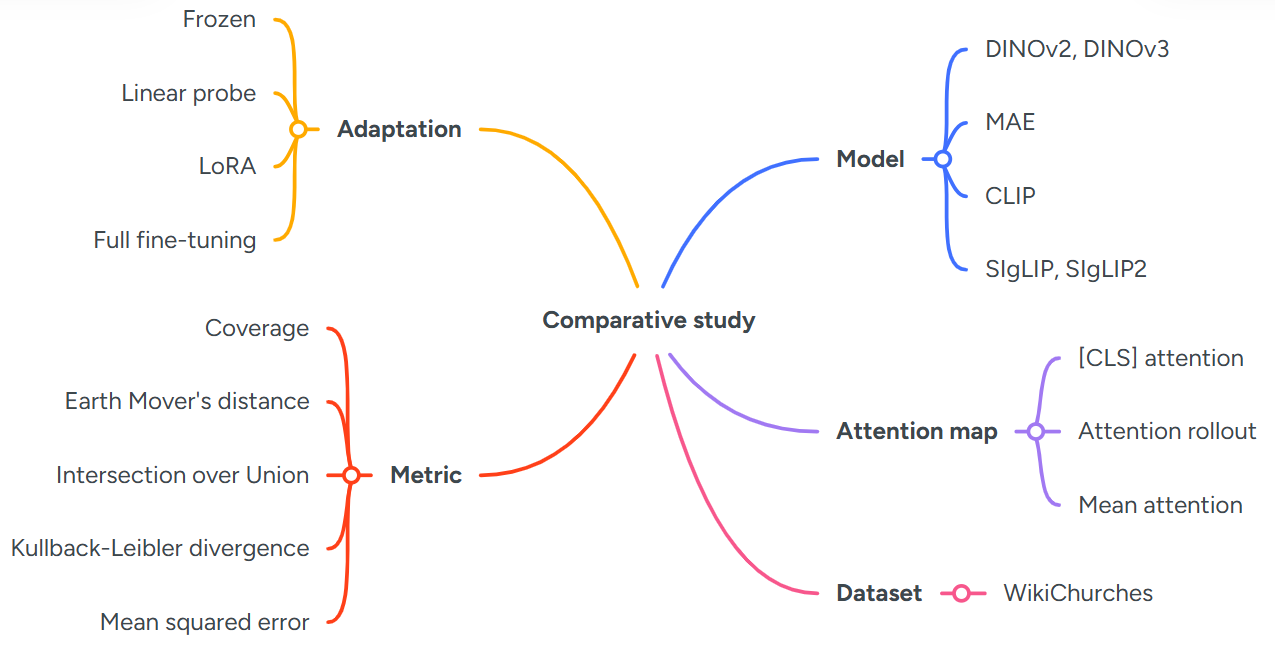
\includegraphics[width=\textwidth]{framework_v1.png}
\caption{A conceptual overview of the experimental pipeline in this study. It compares 6 models, 3 types of attention maps, 4 fine-tuning strategies, and 5 performance metrics on the benchmark WikiChurches dataset. \label{figure framework overview}}
\end{figure}

\subsection{Dataset}

The primary dataset is WikiChurches~\cite{Barz21WikiChurches}, a fine-grained architectural-style dataset of European church buildings. The annotation file defines 106 feature types (arches, windows, towers, portals, etc.) with bounding boxes in normalized coordinates. This project uses two data scopes: (1)~an expert-annotated evaluation subset of 139 images with 631 bounding boxes (Romanesque~51, Gothic~49, Renaissance~22, Baroque~17), and (2)~a larger style-labelled pool from the 9,485-image official release used for fine-tuning. The 139 annotated images are held out from all fine-tuning splits. A key caveat is \textit{sparse annotation bias}: WikiChurches annotates representative instances rather than every visible occurrence of a feature, so a model attending to multiple correct instances may still be penalized by IoU. This is treated as a documented limitation rather than a pipeline defect.

\subsection{Models studied in this paper}

In this paper, we use the term vision foundation models to refer to large pretrained models with general-purpose visual representations. This includes both image-only self-supervised models, such as DINOv2, DINOv3, and MAE, and vision-language models, such as CLIP, SigLIP, and SigLIP2, for which we analyze the visual encoder.

The frozen benchmark compares seven models: six ViT-Base transformers (DINOv2~\cite{Oquab24DINOv2}, DINOv3~\cite{Simeoni26DINOv3}, MAE~\cite{He22MAE}, CLIP~\cite{Radford21CLIP}, SigLIP~\cite{Zhai23SigLIP}, SigLIP2~\cite{Tschannen25SigLIP2}) and ResNet-50 as a supervised CNN baseline. DINOv2 uses patch size~14 with 4 register tokens ($16\!\times\!16$ spatial grid); all others use patch size~16 ($14\!\times\!14$ grid).

Attention extraction depends on architecture (Table~\ref{table attention method list}). \texttt{[CLS]} attention and rollout are used for DINOv2, DINOv3, MAE, and CLIP. SigLIP and SigLIP2 use a mean-attention proxy because they lack an equivalent \texttt{[CLS]}-token pathway. ResNet-50 uses Grad-CAM. These distinctions are especially important in Q3, which is restricted to architecture-native \texttt{[CLS]}-token models.

\begin{table}[!h]
\centering \caption{Attention extraction methods by model family. \label{table attention method list}}
\begin{tabular}{ccc}
\toprule
Attention method & vision foundation model & Remark \\ \midrule
\texttt{[CLS]} attention & DINOv2, DINOv3, MAE, CLIP & Native \texttt{[CLS]} token \\
Rollout & DINOv2, DINOv3, MAE, CLIP & Cross-layer composition \\
Mean attention & SigLIP, SigLIP2 & Proxy (no \texttt{[CLS]} token) \\
\bottomrule
\end{tabular}
\end{table}

Fine-tuning protocols. RQ2 uses a shared experiment-batch workflow. Training is on the non-annotated style-labelled pool with one stratified validation split shared across all model$\times$strategy runs. Best checkpoints are selected by classification validation accuracy; alignment is re-evaluated on the held-out annotated subset. Three strategies are compared (Table~\ref{tab:strategies}); ResNet-50 is excluded from Q2.

\begin{table}[!h]
\centering
\caption{Fine-tuning strategies compared in Q2. \label{table fine tuning list}}
\begin{tabular}{ccc}
\toprule
Strategy & Backbone & Role \\ \midrule
Linear probe & Frozen & Control (zero attention change) \\
LoRA         & Mostly frozen & Efficient adapter \\
Full fine-tuning   & Updated end-to-end & Maximum adaptation \\
\bottomrule
\end{tabular}
\end{table}

\subsection{Performance metrics}

Five metrics are used because no single score suffices for all interpretations.

Let $A$ denote the attention heatmap, $M$ the union binary mask of expert boxes, and $G$ a Gaussian soft-union target derived from the boxes.

\textbf{IoU} thresholds $A$ at the exact top-$k$ pixel count via
\texttt{torch.topk} (top~10\% of pixels) and computes overlap with $M$:
\begin{equation}
  \text{IoU} = \frac{|\hat{A} \cap M|}{|\hat{A} \cup M|}, \quad
  \hat{A} = \text{top-}k\text{-pixels}(A).
\end{equation}
Higher is better.

\textbf{Coverage} is threshold-free: the fraction of total attention energy
inside $M$,
\begin{equation}
  \text{Coverage} = \frac{\sum_{i \in M} A_i}{\sum_i A_i}.
\end{equation}
Higher is better.

\textbf{MSE}, \textbf{KL divergence}, and \textbf{EMD} compare the full
normalised heatmap against $G$. Lower is better for all three.


The study uses paired t-tests, Wilcoxon signed-rank tests, bootstrap confidence
intervals, Cohen's $d$ for paired differences, and Holm multiple-comparison
correction. This is especially important in Q2, where many
model$\times$strategy$\times$metric combinations are compared within shared
correction families.

\subsection{\textcolor{red}{Baselines and calibration}}

\textcolor{red}{TJ: I don't understand why we need this section}

Continuous metrics are calibrated against four naive baselines: random
attention, center Gaussian, saliency prior, and Sobel edge map
(Table~\ref{tab:baselines}). Beating random only is weak evidence; clearing
all four baselines is stronger support for non-trivial semantic alignment.

\begin{table}[h]
\centering
\caption{Dataset-level mean baseline scores (lower is better).}
\label{tab:baselines}
\begin{tabular}{lccc}
\toprule
Baseline & MSE & KL & EMD \\
\midrule
Random         & 0.3192 & 3.3627 & 0.3468 \\
Center Gaussian & 0.1770 & 2.6317 & 0.2836 \\
Saliency Prior & 0.0957 & 2.6111 & 0.2654 \\
Sobel Edge     & 0.0376 & 3.2237 & 0.3137 \\
\bottomrule
\end{tabular}%
\end{table}


\section{Experimental results} \label{section results}

\subsection{Dataset preparation}

\textcolor{red}{TJ: Any \textit{preparation} applied to the dataset? preprocessing? For example, XXX images and xxx annotation instances are used. The box is resized to xxx resolution. }

The 139-image annotated evaluation set spans four architectural styles. Average expert boxes per image are 4.5 overall, but vary by style: Gothic and Romanesque images are more densely annotated (4.2--5.9 boxes/image) than Baroque images (1.8 boxes/image), which limits statistical power for that
subset.

\subsection{Implementation details}

\textcolor{red}{TJ: Need to report all details as much as possible. For example, the DINOv2 model weights are obtained from xxx. During the fine-tuning, it is tuned for the downstream dataset xxx. A linear classifier is added on the frozen backbone, and it is tuned using the optimizer AdamW with cosine learning rate scheduling and early stopping on validation accuracy, and trained for xxx epochs. The LoRA adapter is implemented using xxx parameters, attached to the xxx layer. All experiments are implemented using PyTorch XXX version, a server with XXX CPU, XXX GPU. }

All ViT models use ViT-Base scale. Fine-tuning used AdamW with cosine learning rate scheduling, early stopping on validation accuracy. LoRA adapters are inserted into attention projection layers. Heatmaps are computed at a standardised resolution and cached to HDF5/SQLite for fast backend serving. IoU@90 denotes IoU at the top-10\% pixel threshold. Directions: higher is better for IoU and Coverage; lower is better for MSE, KL, and EMD. Results are reported at each model's best default-method layer over the 139 annotated images.

\subsection{Results from RQ1}

Attention alignment is not one thing. A model can place its strongest attention
inside the expert boxes, spread attention across the right facade region, or
match the overall target distribution - and those are related but not identical
behaviours. Treating one score as the whole answer would make the result look
cleaner than it really is. Instead, RQ1 uses a multi-metric benchmark: IoU@90,
Coverage, MSE, KL divergence, and EMD.

Each metric catches a different failure mode: IoU@90 asks whether the model's
top-attended pixels land inside the expert annotations; Coverage asks what
fraction of total attention energy falls inside the annotated regions; MSE, KL,
and EMD compare the full heatmap against a Gaussian soft-union target, exposing
cases where a model looks reasonable under overlap but still places attention
mass in the wrong location.

Under this benchmark, DINOv3 is the cleanest RQ1 result (Table~\ref{tab:q1}).
It leads on IoU@90, Coverage, KL, and EMD, and is the only model that clears
all four naive baselines on all three continuous metrics. It does not win MSE,
where the extra displayed precision shows SigLIP2 marginally lower than base
SigLIP (0.01745 vs.\ 0.01755) - exactly why the benchmark cannot collapse
to one number. The SigLIP rows also show that \texttt{siglip} and
\texttt{siglip2} should not be treated as interchangeable: base SigLIP
reaches a competitive IoU@90 peak of 0.0739 at \texttt{layer8}, ahead of MAE
and CLIP, while SigLIP2 remains weaker on sharp overlap despite its slightly
lower MSE. SigLIP and SigLIP2 also pair good MSE with EMD~$\approx$~0.35,
worse than the random baseline of 0.3468: smooth local maps can still
misplace attention mass at a distributional level. CLIP's best frozen IoU
occurs at layer~0 rather than in a late-layer regime, consistent with its
global contrastive objective applying no patch-level spatial pressure.

\begin{table}[!h]
\centering
\caption{Results from RQ1 frozen-model alignment leaderboard (best default-method layer, 139 images). $\uparrow$ higher is better; $\downarrow$ lower is better. \label{table RQ1 result}}
\begin{tabular}{cccccc}
\toprule
vision foundation model & IoU $\uparrow$ & Coverage $\uparrow$ & MSE $\downarrow$ & KL divergence $\downarrow$ & EMD $\downarrow$ \\
\midrule
DINOv2    & 0.082 & 0.100 & 0.0209 & 2.684 & 0.298 \\
DINOv3     & \textbf{0.133} & \textbf{0.137} & 0.0270 & \textbf{2.325} & \textbf{0.260} \\
MAE        & 0.070 & 0.090 & 0.0483 & 2.756 & 0.318 \\
CLIP      & 0.049 & 0.085 & 0.0211 & 2.912 & 0.326 \\
SigLIP    & 0.074 & 0.076 & 0.01755 & 3.002 & 0.348 \\
SigLIP2   & 0.047 & 0.071 & \textbf{0.01745} & 3.071 & 0.354 \\
\bottomrule
\end{tabular}
\end{table}

% \begin{figure}[h]
%   \centering
%   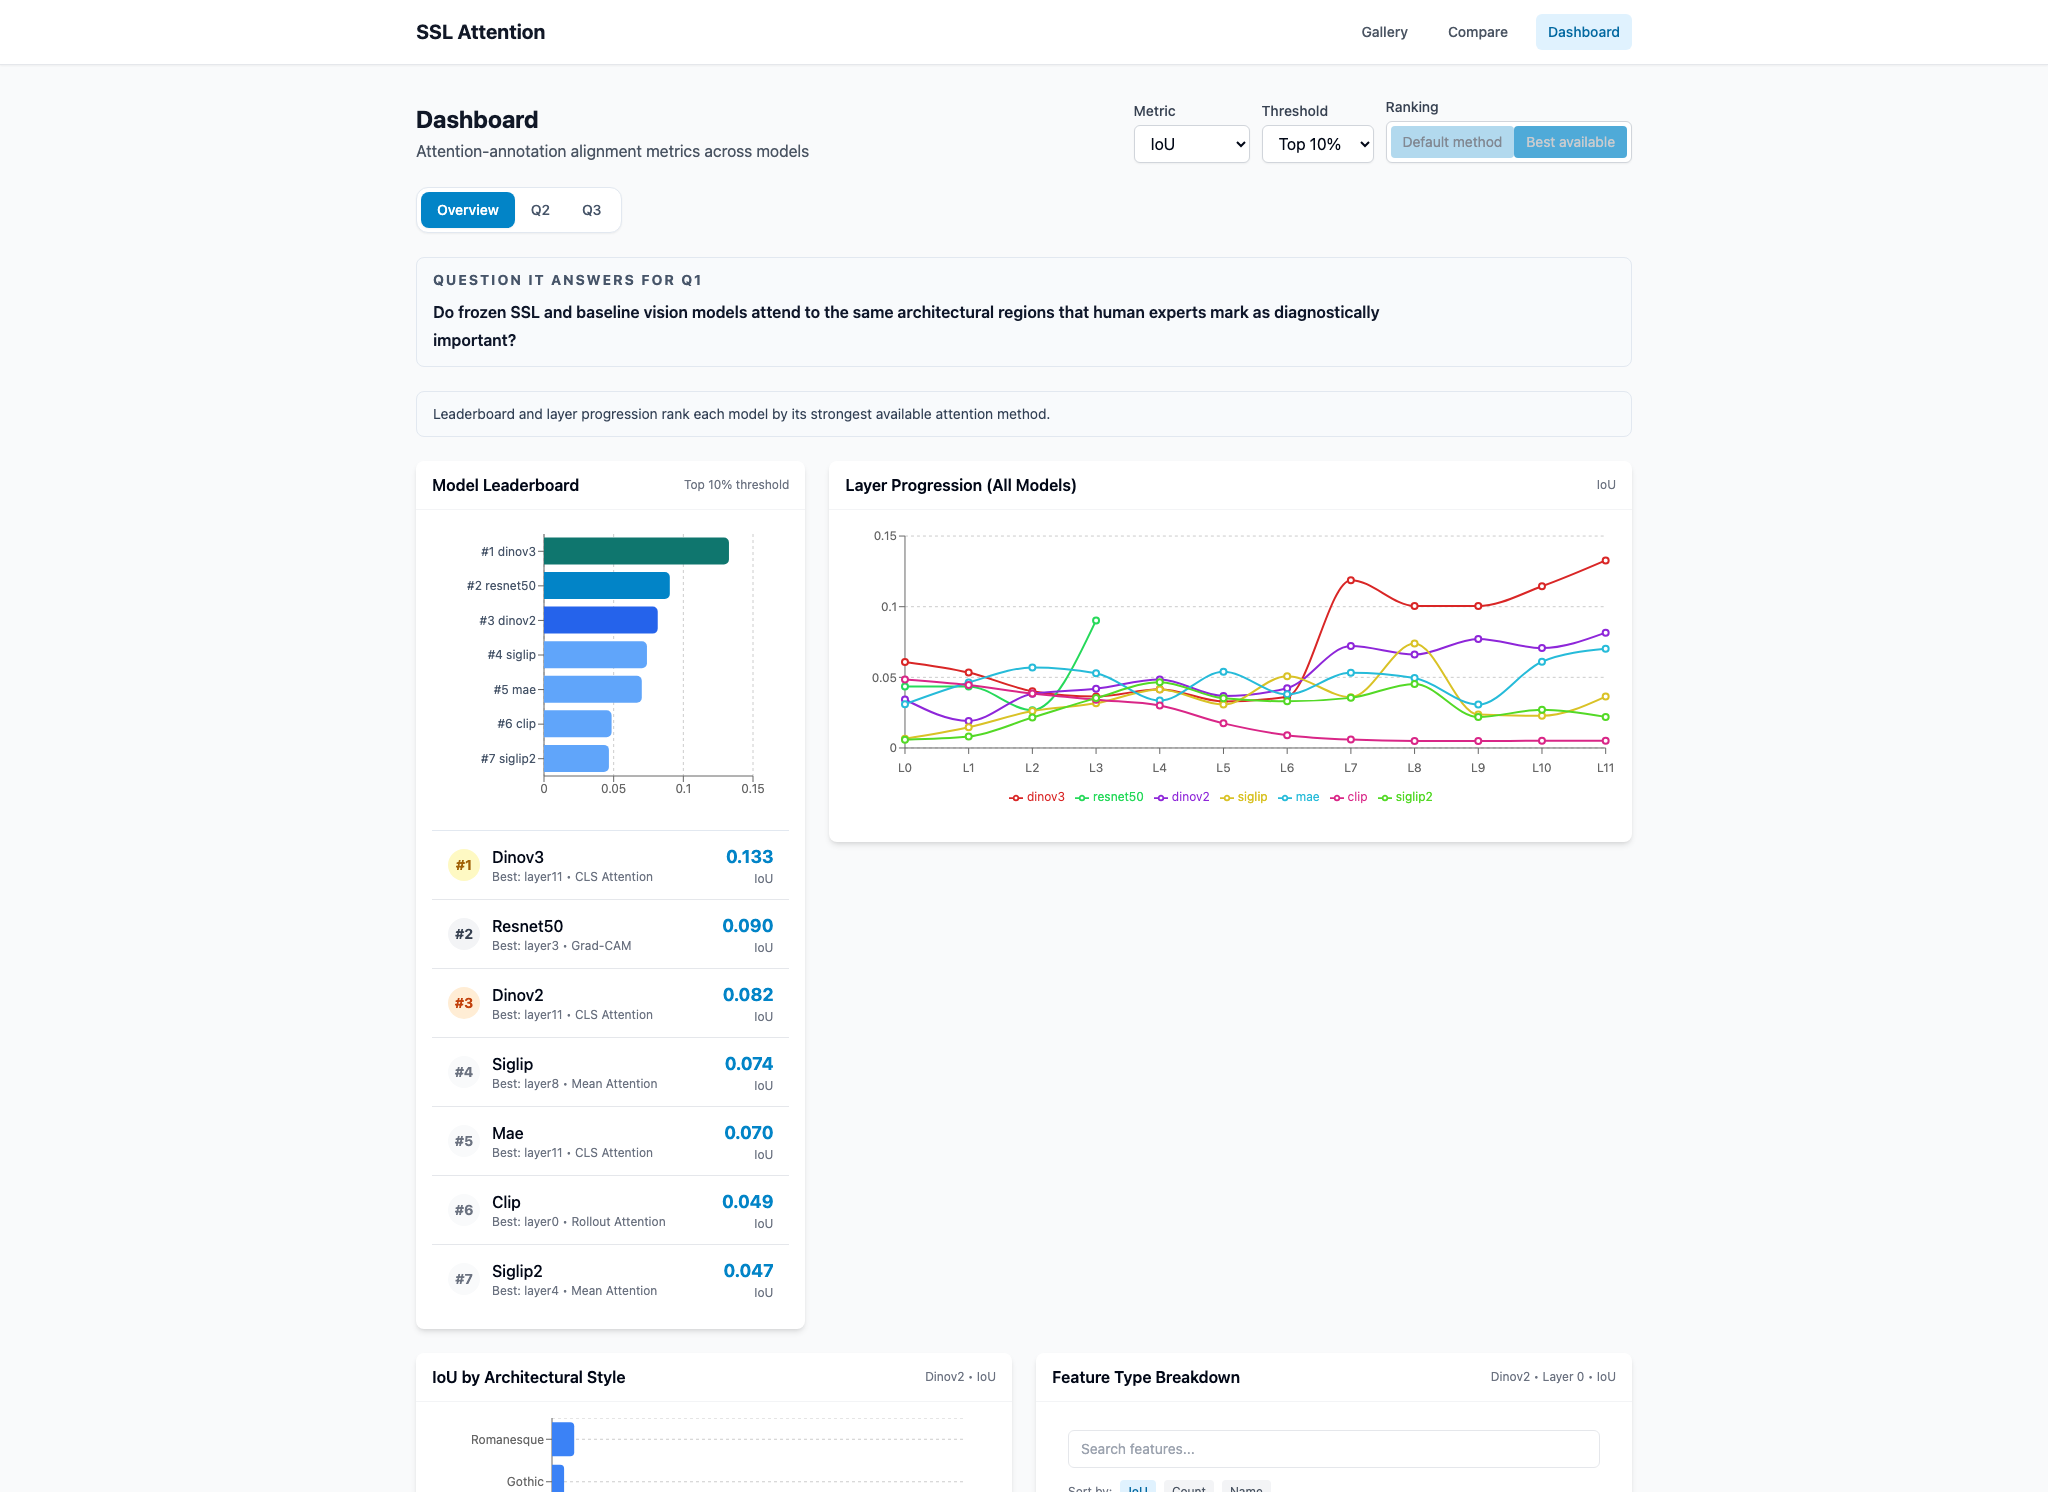
\includegraphics[width=\textwidth]{q1_dinov3_react_dashboard_iou_best_available.png}
%   \caption{React dashboard screenshot (\texttt{/dashboard}, IoU@90, Best available ranking). DINOv3 ranks first at layer~11 with IoU~$=$~0.133 using \texttt{[CLS]} attention. The leaderboard also shows base SigLIP at rank~4 with IoU~$=$~0.074 at \texttt{layer8}, separated from SigLIP2 at rank~7. The layer-progression panel shows DINOv3's late-layer jump relative to other models.}
%   \label{fig:dashboard_q1}
% \end{figure}

Detailed study on DINOv3.

We hypothesize that DINOv3 benefits from the combination of scale, curated data, and a training recipe designed to preserve dense spatial structure. The DINOv3 technical report~\cite{Simeoni26DINOv3} identifies dense-feature degradation as a failure mode during long SSL training and introduces \textbf{Gram anchoring} to stabilise patch-level feature maps. Given that RQ1 metrics reward spatial correspondence to expert-marked architectural parts, a method designed to protect dense features is a natural fit for the observed result.

To corroborate DINOv3's lead, we performed two further checks. The first is robustness: paired image-level tests (Table~\ref{table RQ1 dinov3}) show DINOv3 remains separated from the next-best model on all headline metrics, with Holm-adjusted $p\!<\!1.31\!\times\!10^{-7}$. The second is where DINOv3 wins. If Gram anchoring preserves cleaner patch-level spatial structure, we should expect frozen attention to work best on mid-to-large architectural parts and still struggle on small ornamentation - and that is what we observe.

\begin{table}[!h]
\centering
\caption{RQ1 robustness and spatial checks for DINOv3. \label{table RQ1 dinov3}}
\begin{tabular}{lp{0.4\textwidth}p{0.35\textwidth}}
\toprule
Check & Result & Why it matters \\
\midrule
Paired gap & $+$0.0425 IoU, $+$0.0330 Cov, $+$0.3595 KL, $+$0.0378 EMD & Lead is not a leaderboard artifact \\
Strongest styles & Gothic 0.169, Romanesque 0.160 & Highest where structure is visually prominent \\
Strongest features & Ornate Portal 0.214, Tracery Rose 0.164 & Aligns with large coherent parts \\
Weakest features & Crocket, Fleuron, Pinnacle & Small ornamentation remains hard \\
\bottomrule
\end{tabular}
\end{table}



\subsection{Results from RQ2}

RQ2 defines \emph{descriptive specialisation} as a head whose \texttt{[CLS]}-to-patch attention map consistently aligns better than other heads with expert-marked regions or feature labels. It is not a causal-attribution claim. The scope is the architecture-native \texttt{[CLS]}-token ViTs: DINOv2, DINOv3, MAE, and CLIP; SigLIP, SigLIP2, and ResNet-50 are excluded because their per-head proxies do not use native attention heads, and rollout is excluded because it aggregates layers. Heads are ranked primarily by IoU@90, with Coverage and EMD as robustness checks.

\subsubsection{A study on various layers}

\begin{figure}[!h]
\centering
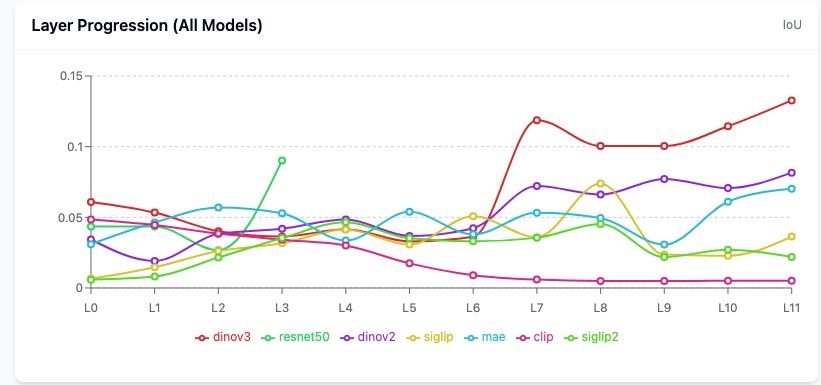
\includegraphics[width=\linewidth]{RQ2_layer_iou.png}
\caption{Layer ranking}
\label{figure RQ3 layer ranking}
\end{figure}


\subsubsection{Head-Feature Matrix.}

Head Ranking identifies a dominant head shown in Figure \ref{figure RQ2 feature matrix}; the Head-Feature Matrix asks what architectural evidence that head aligns with. The observation is that the strongest heads mostly align with larger, coherent structural features. For DINOv3, the same \texttt{layer10/head8} that leads the ranking view also carries the selected \emph{Columned Portal} cell at IoU@90~$=$~0.215 across 15 annotations, linking the ranking evidence to the feature evidence.

\begin{figure}[!h]
\centering
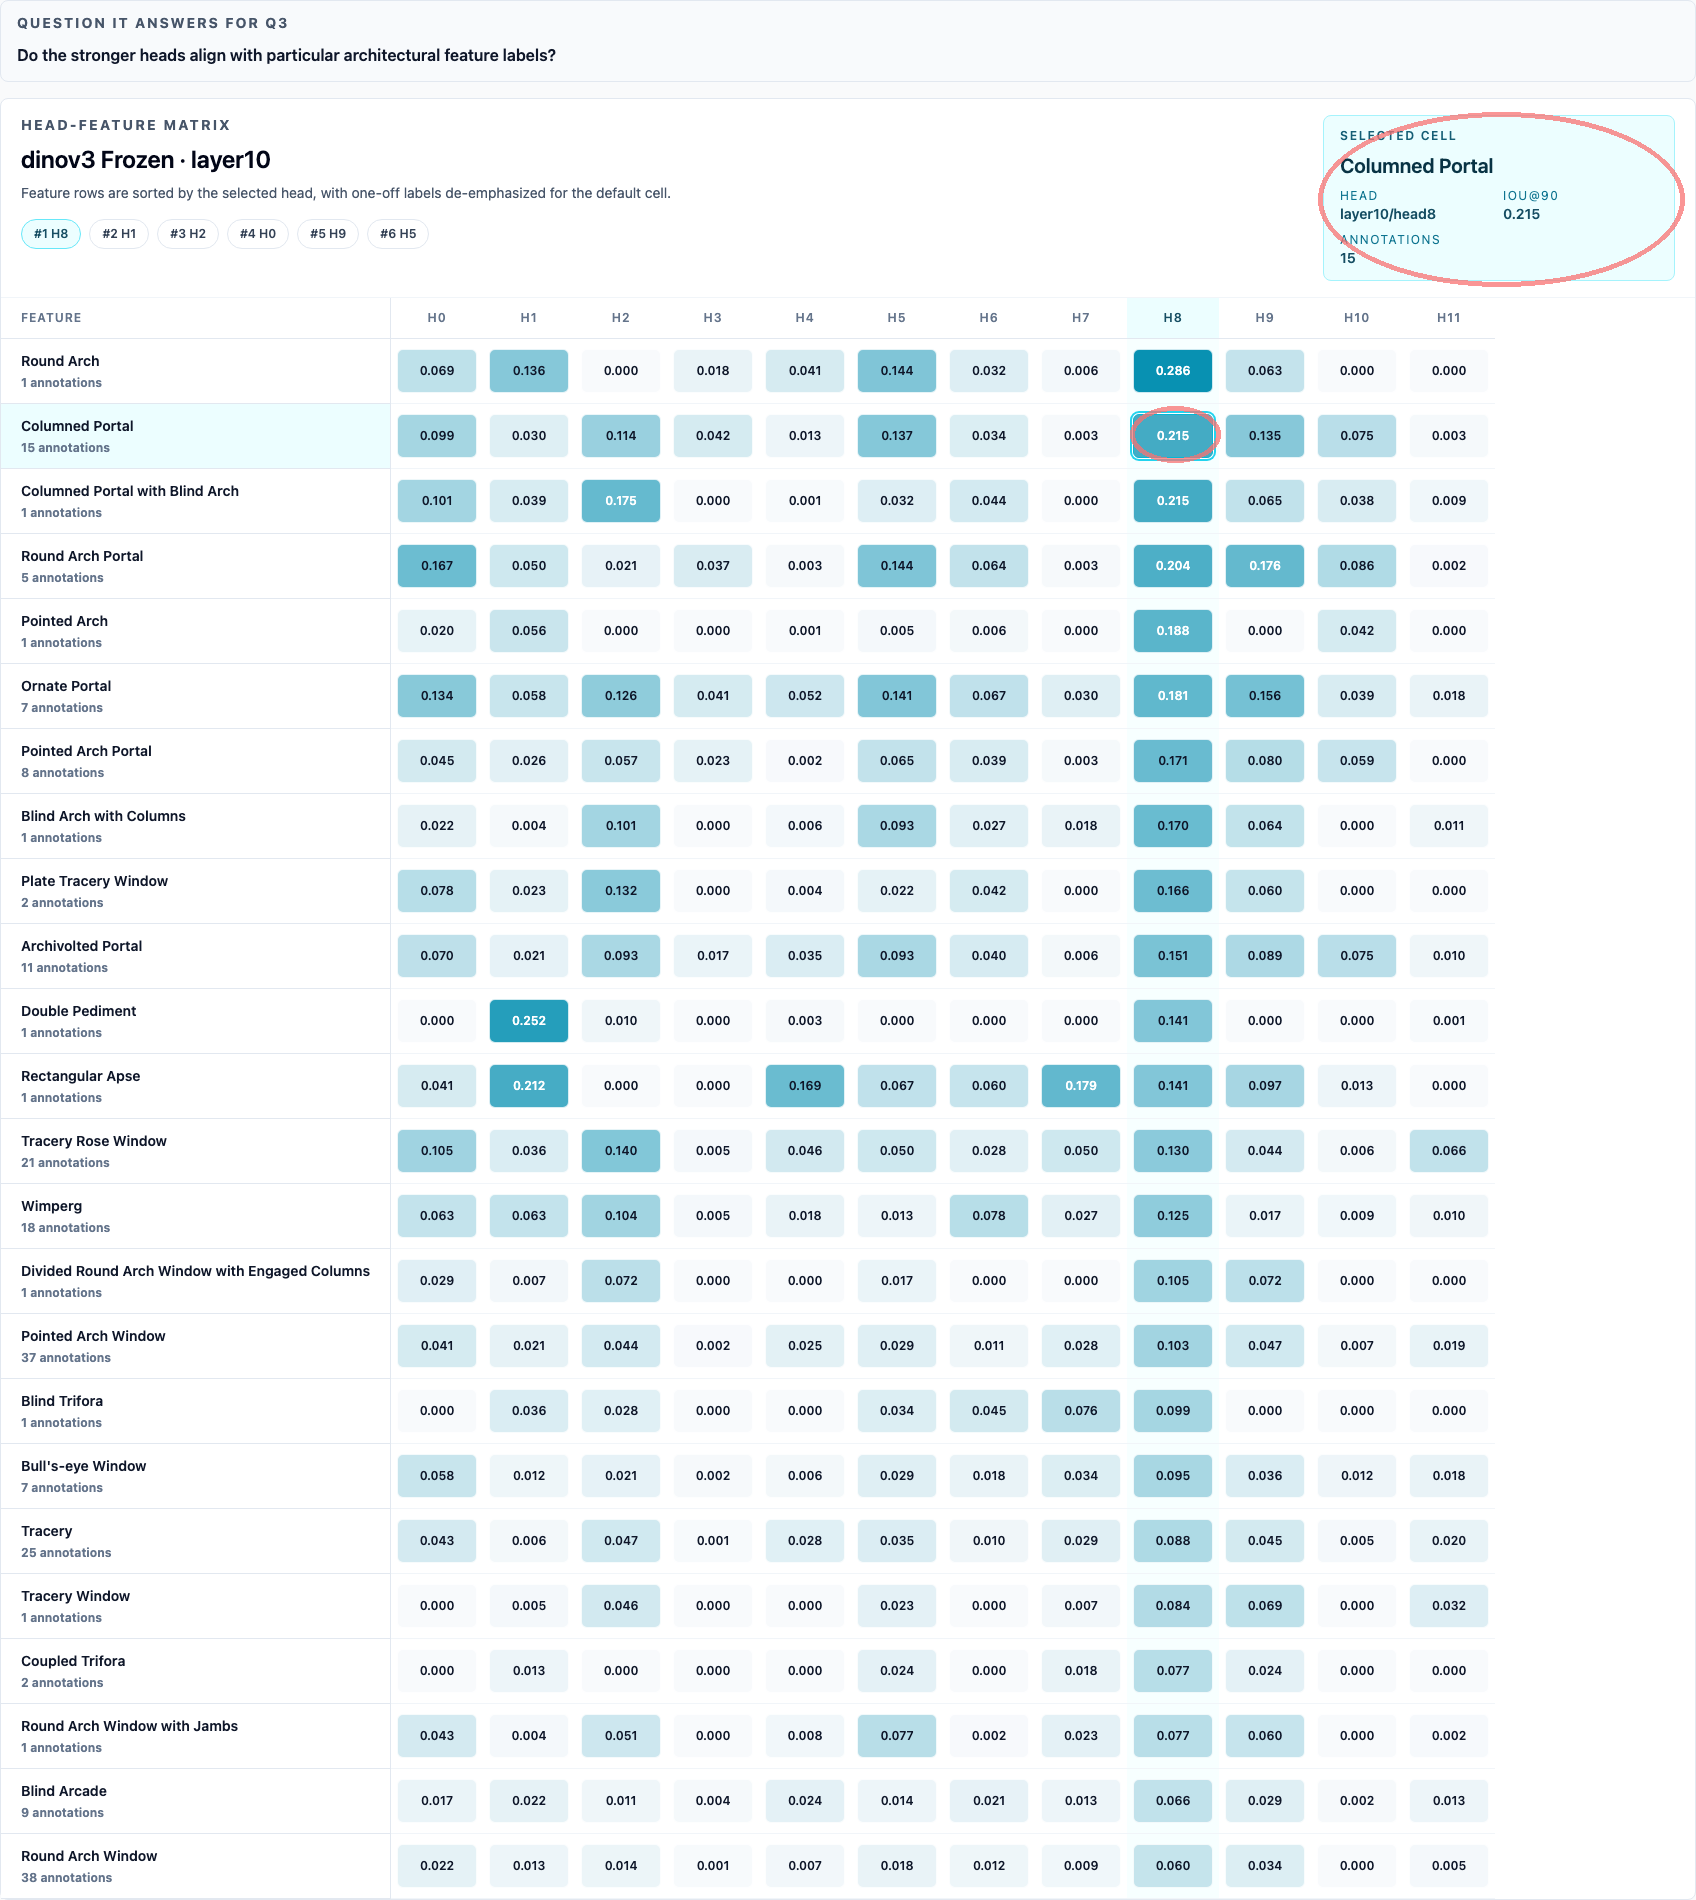
\includegraphics[width=\textwidth]{RQ2_head_feature_matrix_report_view.png}
\caption{RQ2. Head-Feature Matrix report view for DINOv3 frozen attention
(\texttt{layer = 10}, IoU@90). The same \texttt{head8} that leads the
ranking view also carries the selected \emph{Columned Portal} cell at
IoU@90~$=$~0.215 across 15 annotations: the dominant head is strongest on
portal-scale structure.}
\label{figure RQ2 feature matrix}
\end{figure}

To keep the visual check disciplined, for each scoped RQ3 model, we take its frozen IoU@90 dominant head from the ranking view and sort architectural features for that head with at least three annotations. Figure~\ref{figure RQ2 top bottom} shows the three strongest and three weakest
features for each model's dominant head.

\begin{figure}[!h]
\centering
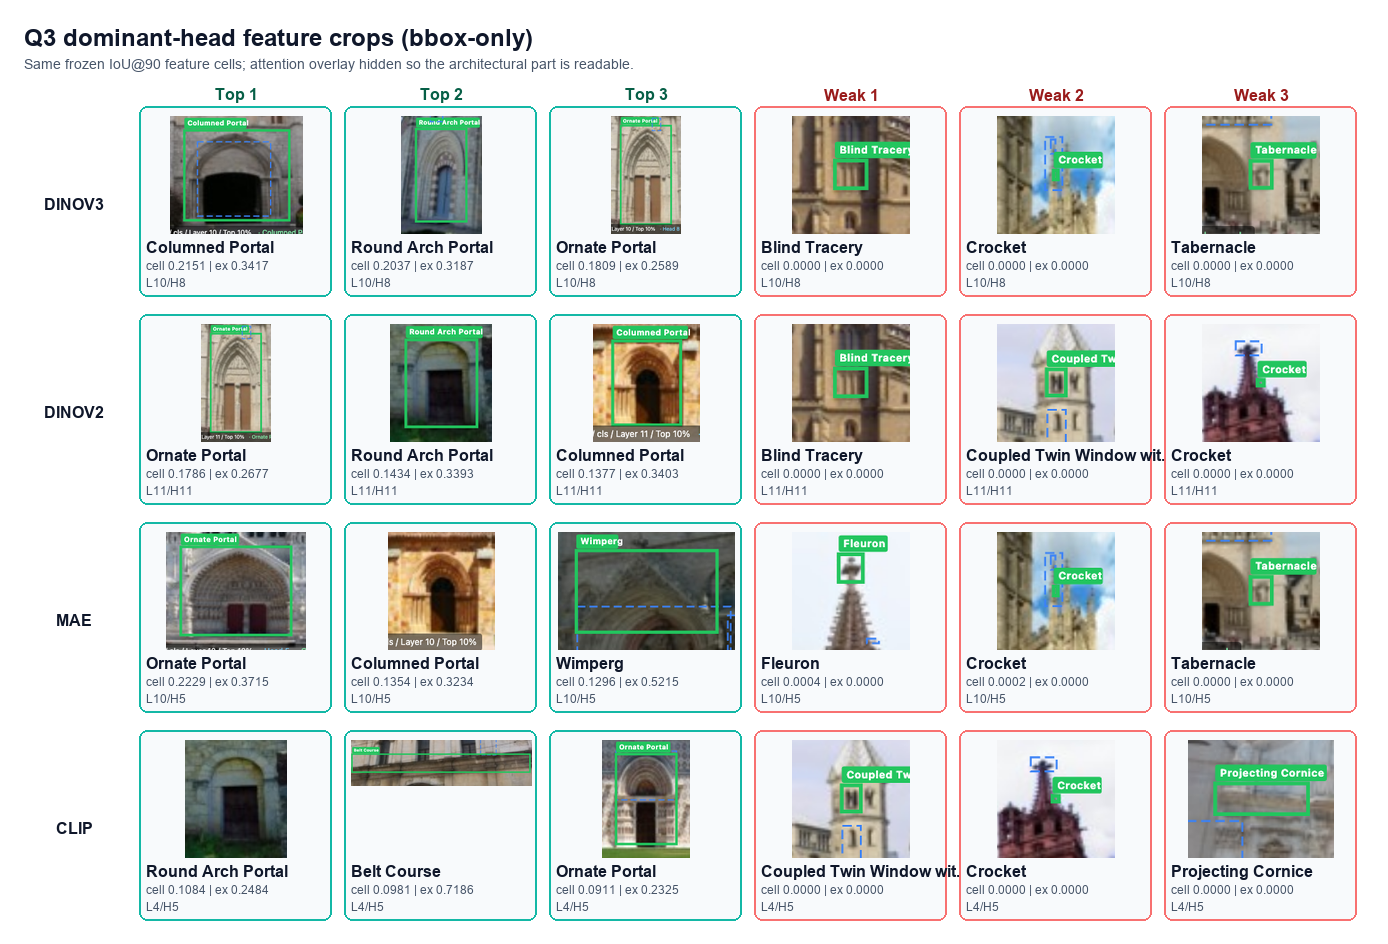
\includegraphics[width=\textwidth]{RQ2_head_feature_top_bottom_contact_sheet.png}
\caption{Frontend Image Detail RQ3 crops for the frozen dominant IoU@90 head in each scoped model: DINOv3 \texttt{layer10/head8}, DINOv2 \texttt{layer11/head11}, MAE \texttt{layer10/head5}, CLIP
\texttt{layer4/head5}. Strongest features are dominated by portal-scale or facade-structure parts (\emph{Columned Portal}, \emph{Round Arch Portal}, \emph{Ornate Portal}, \emph{Wimperg}, \emph{Belt Course}). Weakest features are thin or decorative labels (\emph{Blind Tracery}, \emph{Crocket}, \emph{Tabernacle}, \emph{Fleuron}, \emph{Coupled Twin Window with Discharging Arch}, \emph{Projecting Cornice}).}
\label{figure RQ2 top bottom}
\end{figure}

Across the four scoped models, the pattern is consistent. DINOv3's \texttt{layer10/head8} reaches mean feature-level IoU@90 of 0.215 on \emph{Columned Portal}, 0.204 on \emph{Round Arch Portal}, and 0.181 on \emph{Ornate Portal}, while its weakest supported features are essentially zero on \emph{Blind Tracery}, \emph{Crocket}, and \emph{Tabernacle}. DINOv2 shows the same portal-heavy top end and the same small-detail failure boundary. MAE also favours large facade parts, but its third-strongest feature is \emph{Wimperg}, fitting the RQ2 observation that MAE is more responsive to compact geometric forms. CLIP's inclusion of \emph{Belt Course} suggests feature extent and clean geometry matter, not only semantic category names.

The strongest heads are therefore better described as heads whose spatial patterns are more compatible with expert-marked \emph{structural} parts rather than as exact part detectors, and the failure cases are not random: across families, the weak features tend to be small, thin, repeated, or visually entangled with surrounding masonry.

One caveat moderates the weak-feature reading. IoU@90 keeps a fixed-size top-10\% attention region and scores it against a variable-size expert mask, so for thin or repeated ornamentation (\emph{Crocket}, \emph{Fleuron}, \emph{Blind Tracery}), the mask is small, and the achievable IoU@90 is mechanically capped regardless of where attention falls. Part of the weak-feature shortfall is therefore metric geometry rather than head-attribution; a threshold-free Coverage check would help separate the two effects.

% \subsubsection*{Frozen-to-Adapted Delta.}

% Head Ranking shows whether the winning head changes across variants. The Frozen-to-Adapted Delta view asks the sharper follow-up: when adaptation changes the dominant head, does the strongest expert-aligned signal stay in the same head or move to a different one? Here, \emph{expert-aligned signal} means the selected head's normalised \texttt{[CLS]}-to-patch heatmap scored against expert boxes; for IoU@90 the pipeline keeps the top 10\% of heatmap pixels and compares that binary mask with the expert-box union, and the head with the highest mean IoU@90 across the 139 images is treated as the strongest expert-aligned head for that layer, variant, and metric.

% The answer is family-specific: DINO-family heads are mostly preserved, MAE is partially reshaped, and CLIP shows the clearest reorganisation. The delta view makes the CLIP case concrete inside \texttt{layer11}, the late layer where adapted CLIP becomes strongest. The cross-layer change is that frozen CLIP's best alignment lives in early layers (\texttt{layer4} max IoU@90~$=$~0.067), while \texttt{layer11} is weak before adaptation (0.034 max). Adaptation strengthens \texttt{layer11} (0.084 LoRA, 0.105 Full) without substantially changing \texttt{layer4/head5}; this view then zooms into \texttt{layer11} to show which adapted heads pick up the new signal: frozen \texttt{H4} gives way to LoRA \texttt{H11} and Full \texttt{H3} (Figure~\ref{fig:q3_delta}).

% \begin{figure}[h]
% \centering
% 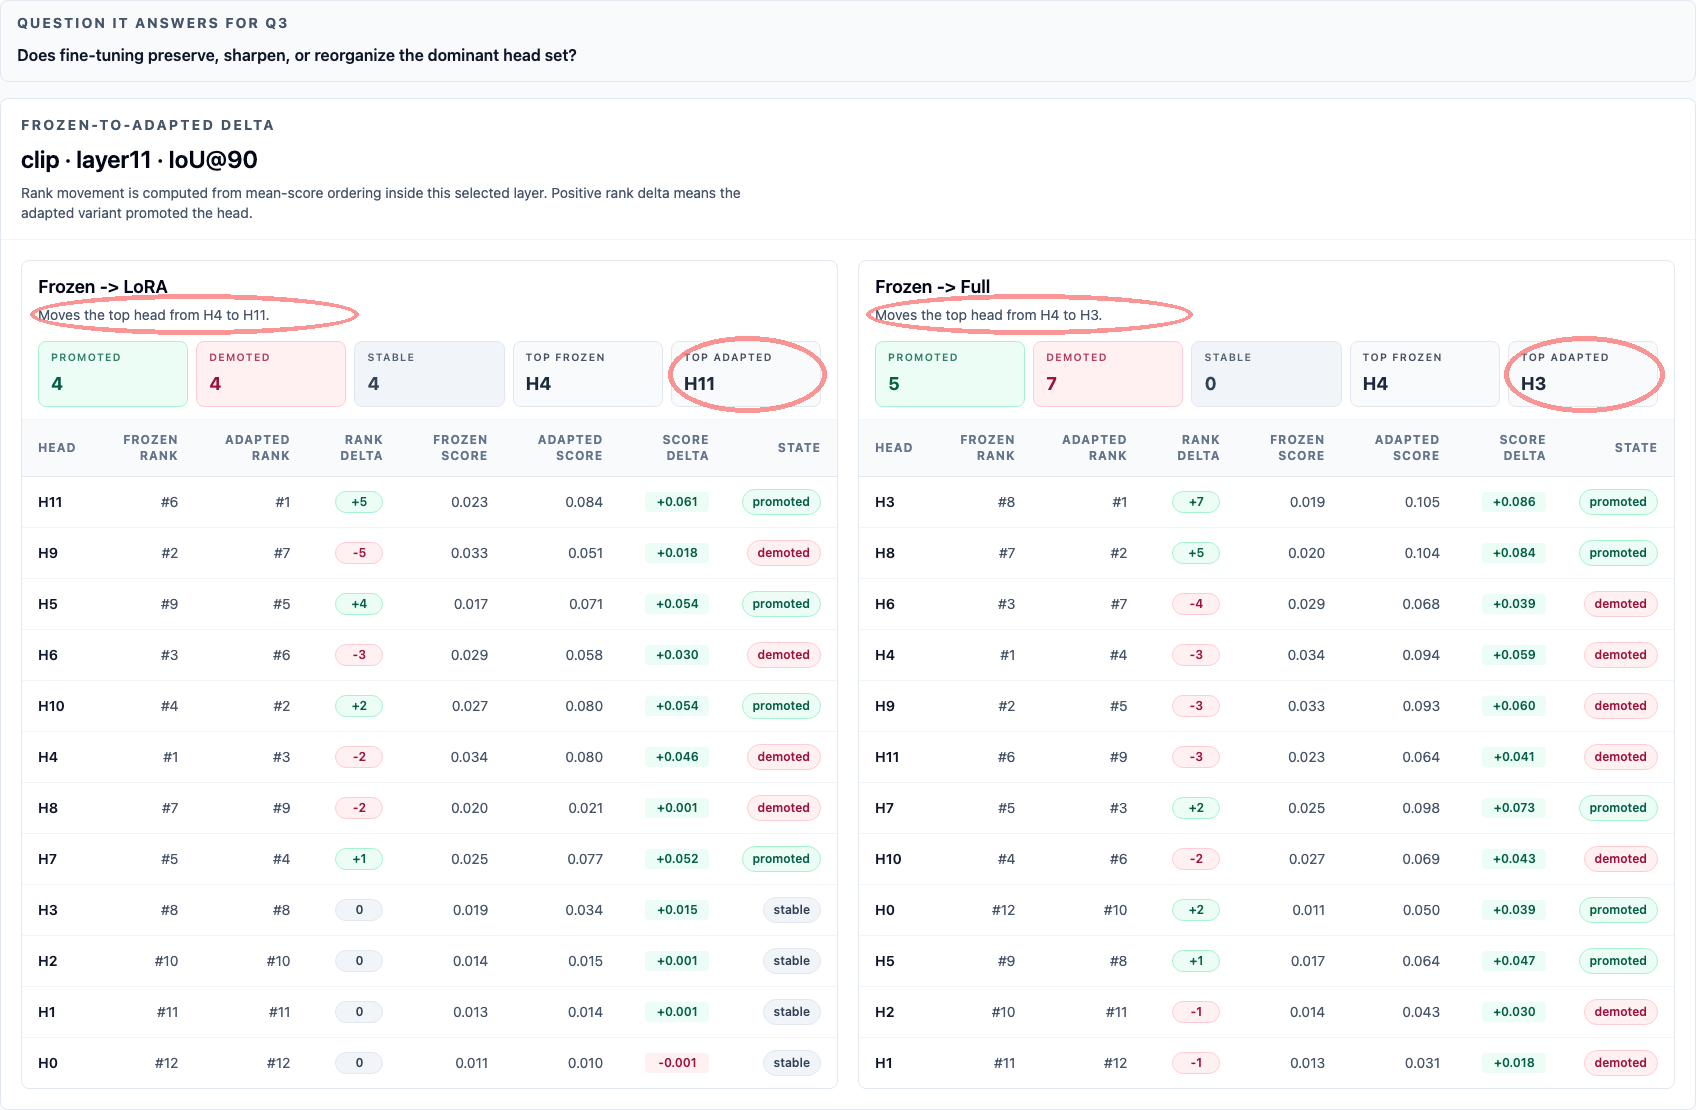
\includegraphics[width=\textwidth]{q3_frozen_adapted_delta_report_view.png}
% \caption{Frozen-to-Adapted Delta report view for CLIP (\texttt{layer = 11},
% IoU@90). Within the same late layer, the LoRA comparison moves the top head
% from \texttt{H4} to \texttt{H11}, while the Full comparison moves it from
% \texttt{H4} to \texttt{H3}.}
% \label{fig:q3_delta}
% \end{figure}

% Reading the four scoped models together: DINOv3 is the clean stability case, with \texttt{layer10/head8} remaining the strongest IoU@90 head in Frozen, LoRA, and Full and top-3 support above 110/139 images in every condition; DINOv2 shows the same preserved-head pattern at lower absolute alignment with \texttt{layer11/head11}. MAE is the intermediate case - Frozen and Full both favour \texttt{layer10/head5}, while LoRA shifts the strongest IoU@90 head to \texttt{layer11/head7}: not a full CLIP-style rewrite, but evidence that parameter-efficient adaptation can move MAE's dominant signal. CLIP is the clearest reorganisation case: in \texttt{layer11}, LoRA promotes \texttt{H11} from rank \#6 to \#1, with frozen-best \texttt{H4} only falling to \#3 and remaining close in score (0.080 vs.\ 0.084), so LoRA promotes a new top head without erasing the frozen late-layer pattern. Full fine-tuning reorganises CLIP more strongly - \texttt{H3} moves from \#8 to \#1, \texttt{H8} moves from \#7 to \#2, and frozen-best \texttt{H4} drops to \#4. Read with Head Ranking, this gives the CLIP-specific claim: adaptation strengthens expert alignment in \texttt{layer11} (where frozen CLIP is weak, 0.034 max) and reorganises the within-layer ranking of those newly strengthened heads. DINO-style models already align well with expert regions before fine-tuning, so adaptation leaves their strongest heads mostly unchanged. CLIP and MAE have more room to move: after adaptation, the best-aligned attention comes from \emph{different heads}, not just from the same head with a higher score.

\subsection{Results from RQ3}

Linear Probe produces exactly zero $\Delta$ across all metrics for all models, confirming that observed RQ3 movement is tied to actual representation change rather than a reporting artefact. Figure~\ref{figure RQ3 heatmap} shows the multi-metric improvement heatmap across all non-Linear-Probe combinations. Figure~\ref{figure RQ3 forest} adds the statistical layer with bootstrap confidence intervals.

\begin{figure}[!h]
\centering
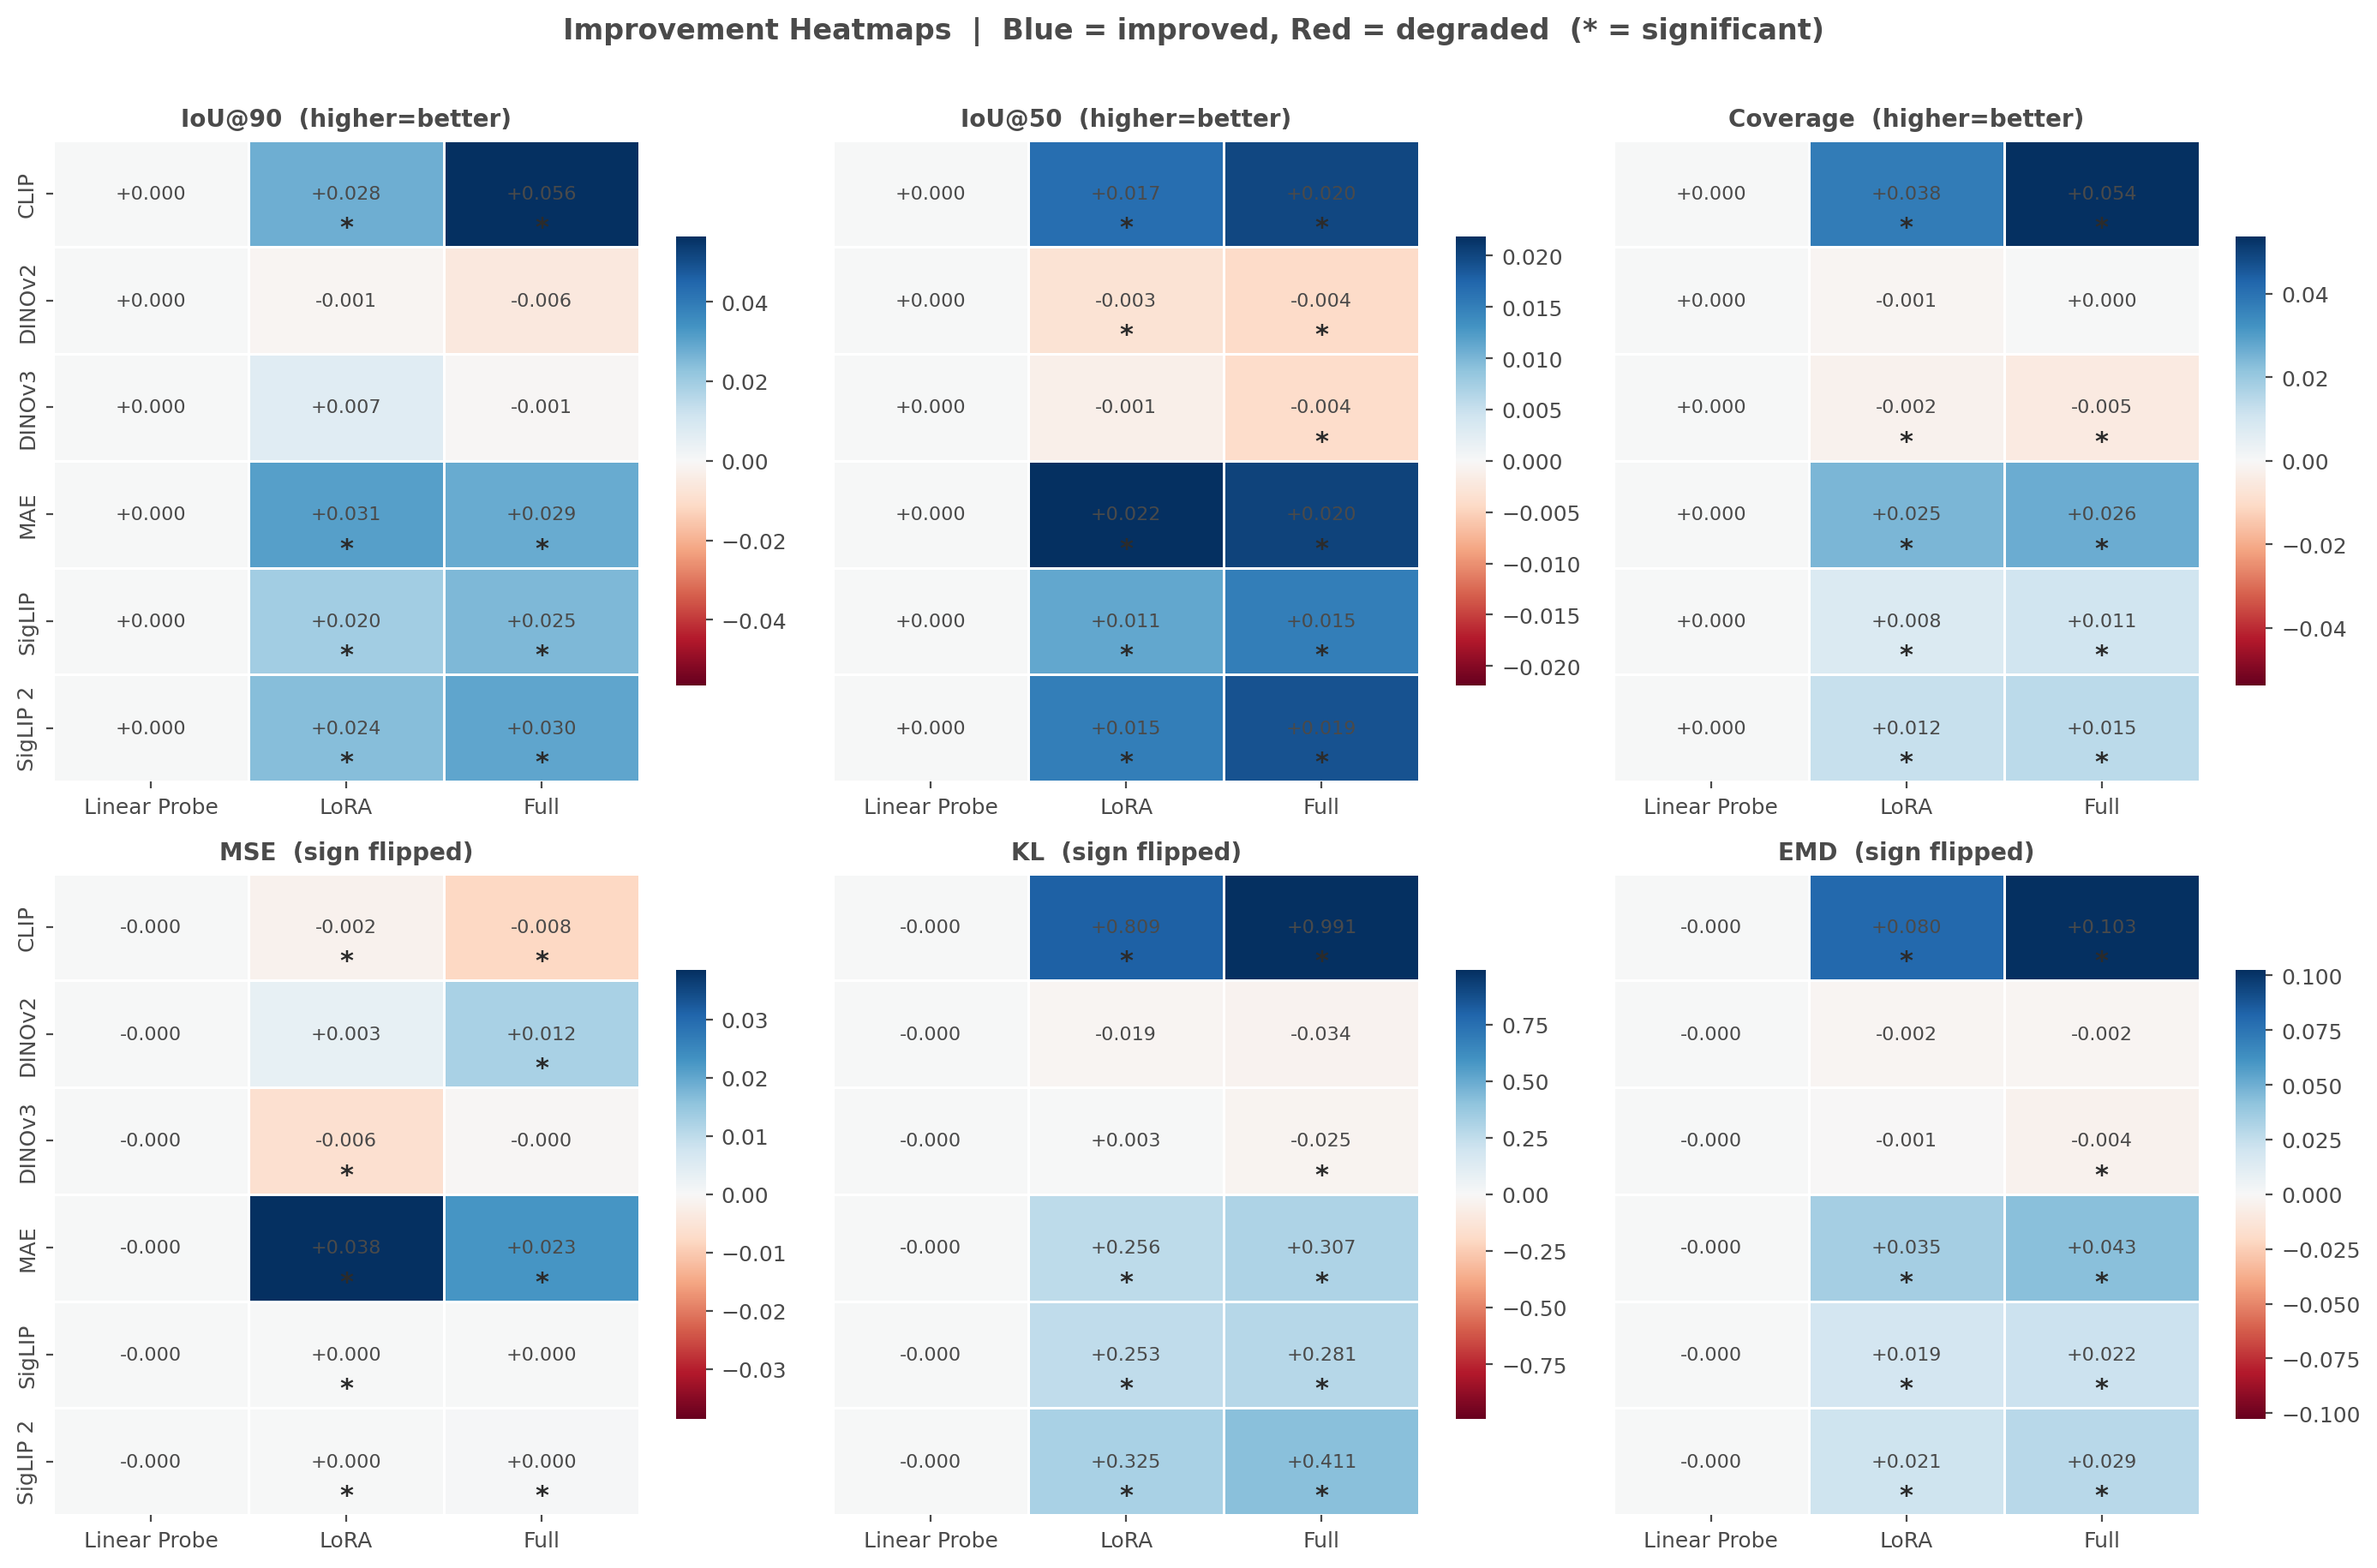
\includegraphics[width=\textwidth]{RQ3_all_metrics_improvement_heatmap.png}
\caption{Q2 multi-metric improvement heatmap. Each cell shows whether LoRA or Full fine-tuning enhances, preserves, or degrades alignment relative to the frozen model. \textcolor{red}{TJ: all results use the same order, DINOv2, DINOv3, MAE, CLIP, SIgLIP, SIgLIP2. Enlarge text fonts. Enlarge the height of the right legend bar}}
\label{figure RQ3 heatmap}
\end{figure}


\begin{figure}[!h]
\centering
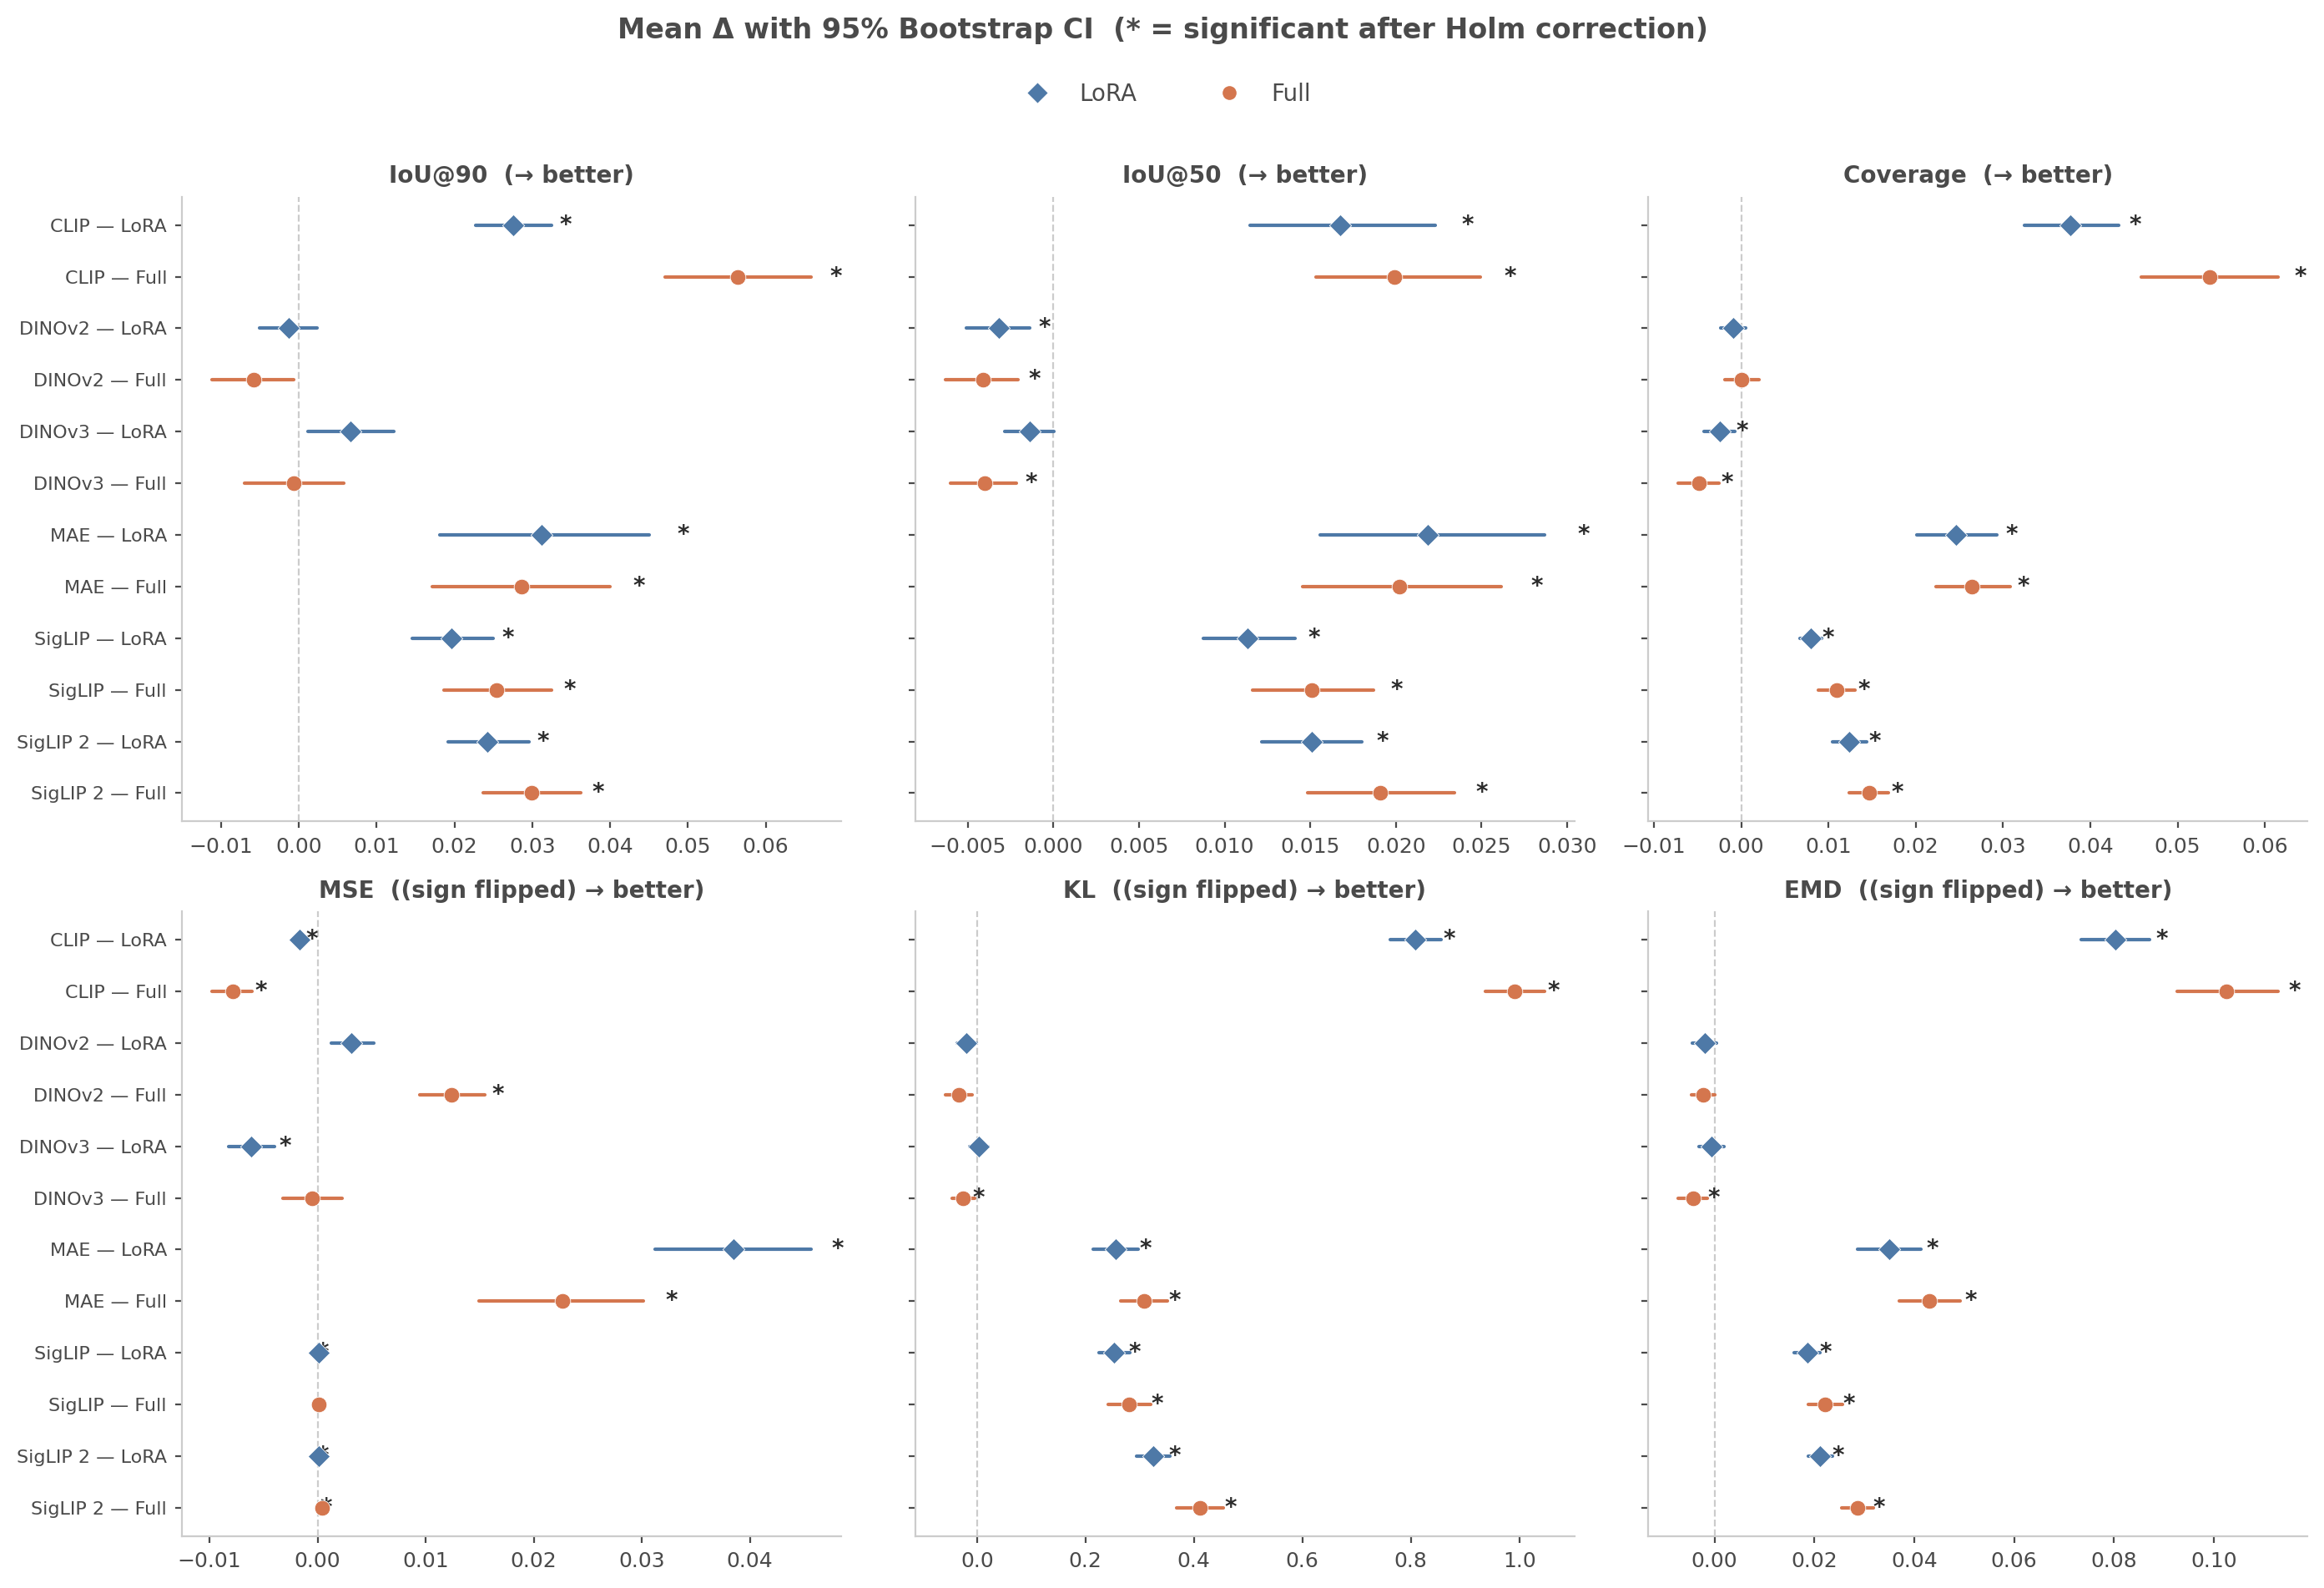
\includegraphics[width=\textwidth]{RQ3_forest_plot_ci.png}
\caption{Forest plot of $\Delta$IoU@90 with 95\% bootstrap confidence intervals per model and strategy.}
\label{figure RQ3 forest}
\end{figure}

\begin{table}[!h]
\centering
\caption{Per-style $\Delta$IoU@90 under Full fine-tuning.}
\label{table RQ3 perstyle}
\begin{tabular}{lcccc}
\toprule
Vision foundation model & Romanesque & Gothic & Renaissance & Baroque \\ \midrule
DINOv2  & $-$0.010 & +0.001 & $-$0.004 & $-$0.012 \\
DINOv3  & $-$0.001 & +0.006 & $-$0.004 & $-$0.009 \\
CLIP    & +0.066 & +0.079 & +0.014 & +0.013 \\
MAE     & +0.007 & +0.009 & +0.108 & +0.045 \\
SigLIP2 & +0.034 & +0.044 & +0.007 & +0.007 \\
SigLIP  & +0.029 & +0.039 & $-$0.006 & +0.005 \\
\bottomrule
\end{tabular}
\end{table}


CLIP shows the largest gain (Full fine-tuning: IoU $0.0181\!\to\!0.0745$, Coverage $0.051\!\to\!0.105$, Cohen's $d\!\approx\!1.0$). The per-style breakdown (Table~\ref{table RQ3 perstyle}) reveals that virtually all of CLIP's gain concentrates on Romanesque (+0.066) and Gothic (+0.079) images, whose diagnostic features (Round Arch Portals, Pointed Arch Portals, Tracery) appear frequently in English-language web text - consistent with CLIP's language-grounded training. Renaissance (+0.014) and Baroque (+0.013) show near-zero gain.

A Kruskal-Wallis test finds significant style moderation for CLIP ($p\!=\!7.2\!\times\!10^{-9}$), MAE ($p\!=\!3.8\!\times\!10^{-7}$), SigLIP ($p\!=\!1.5\!\times\!10^{-5}$), and SigLIP2 ($p\!=\!5.0\!\times\!10^{-7}$); DINOv2 and DINOv3 are not significant ($p\!=\!0.18$, $p\!=\!0.12$), consistent with their near-zero per-style profiles.

\textbf{MAE}'s Renaissance $\Delta$ of +0.108 is the largest single-style shift in the dataset. The two most common Renaissance features (Pilaster, Belt Course) show negative $\Delta$, suggesting the style-classification gradient routes attention toward the most discriminative geometric forms.

% \begin{table}[h]
% \centering
% \caption{Per-feature $\Delta$IoU for MAE (Full fine-tuning, Renaissance images).}
% \label{tab:mae_renaissance}
% \begin{tabular}{lccc}
% \toprule
% Feature & Froz.\ IoU & FT IoU & $\Delta$IoU \\
% \midrule
% Triangular Pediment & 0.036 & 0.116 & +0.080 \\
% Cranked Cornice     & 0.005 & 0.067 & +0.062 \\
% Broken Pediment     & 0.005 & 0.060 & +0.055 \\
% Volute              & 0.009 & 0.052 & +0.043 \\
% Segmental Pediment  & 0.013 & 0.054 & +0.042 \\
% Pilaster            & 0.023 & 0.011 & $-$0.012 \\
% Belt Course         & 0.031 & 0.015 & $-$0.016 \\
% \bottomrule
% \end{tabular}
% \end{table}

\textbf{SigLIP variants.} \textcolor{red}{TJ: which figure/table is used to get this analysis?} The RQ2 analysed layer is \texttt{layer11}, where both SigLIP and SigLIP2 start from weaker frozen IoU@90 baselines than the DINO family (\texttt{siglip} 0.0364, \texttt{siglip2} 0.0220). Under Full fine-tuning, base SigLIP remains higher in absolute IoU@90 (0.0618 vs.\ SigLIP2 0.0519), but SigLIP2
moves further in standardised-effect terms ($\Delta\!=\!0.0299$, Cohen's $d\!=\!0.781$, vs.\ SigLIP's $\Delta\!=\!0.0254$, $d\!=\!0.604$), consistent with more late-layer adaptation headroom from a weaker starting point and the denser grounding components of SigLIP2.

\textbf{DINO family.} Both DINOv2 and DINOv3 show near-zero $\Delta$ across all styles and strategies. $\Delta\!\approx\!0$ is a positive generalisation result: expert-aligned spatial structure is already encoded by pretraining, and the style-classification gradient is absorbed by the classification head rather than reshaping backbone attention.


% \begin{figure}[t]
%   \centering
%   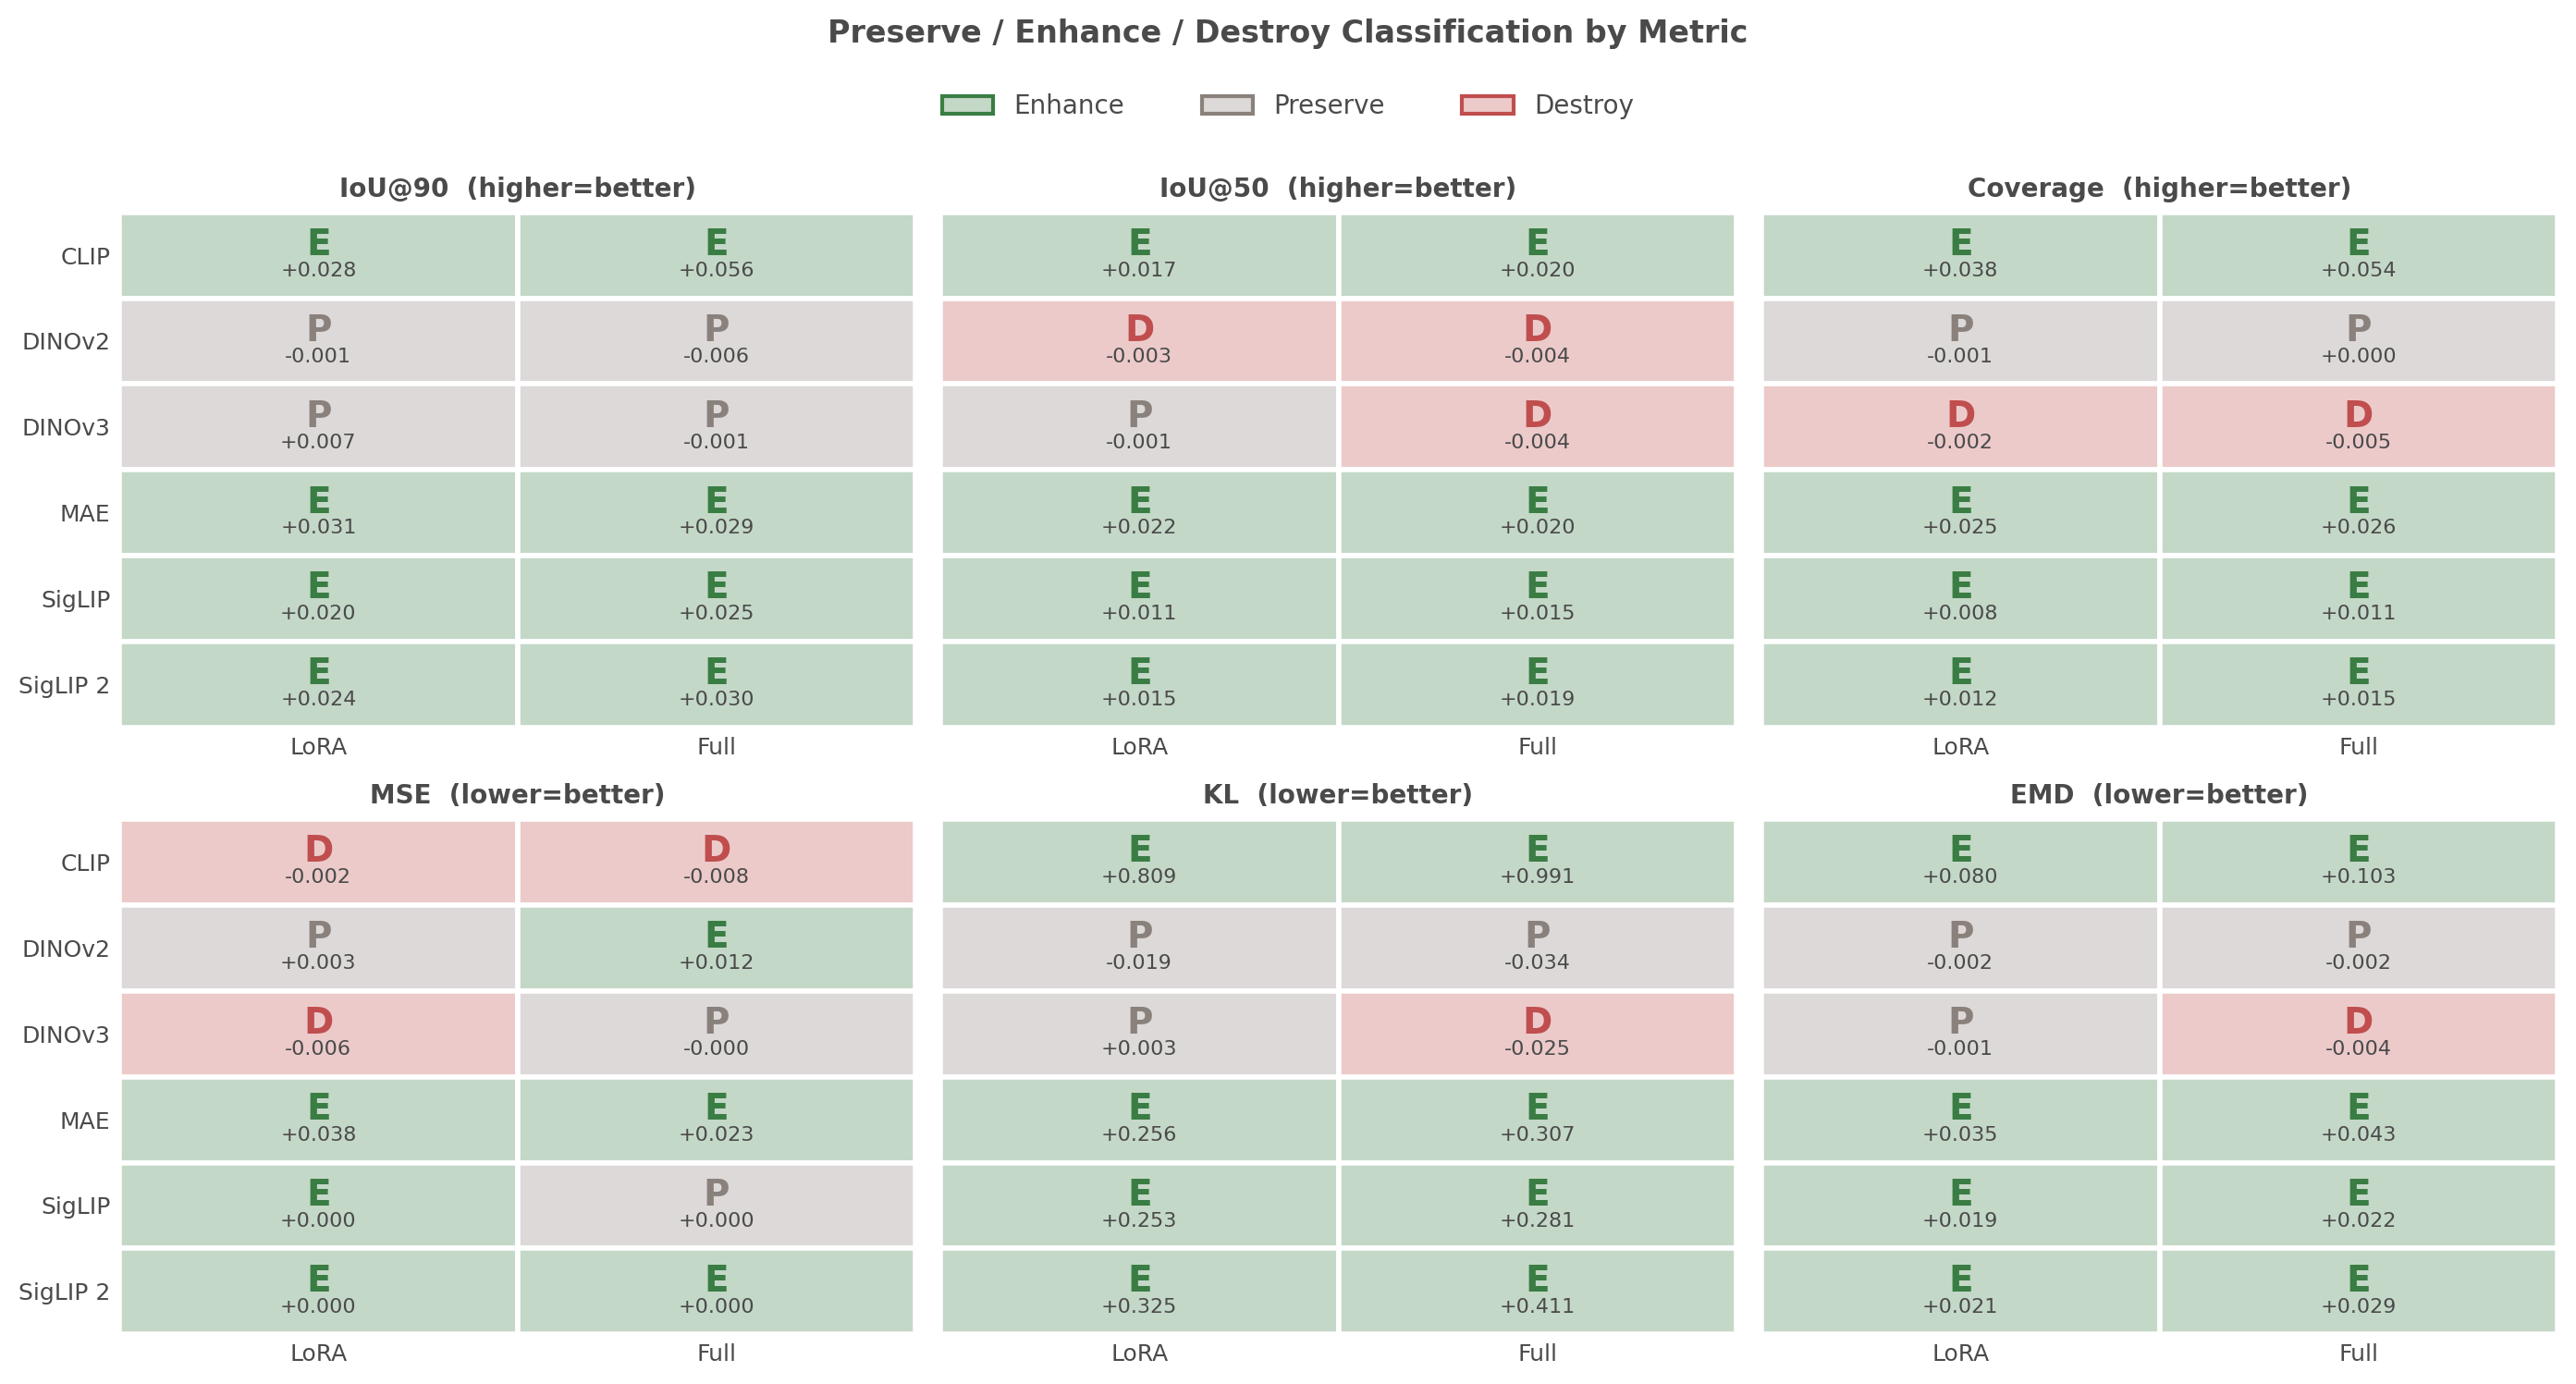
\includegraphics[width=\textwidth]{07_preserve_enhance_destroy.png}
%   \caption{Preserve/enhance/destroy classification across 72 non-LP combinations. Fine-tuning dominantly enhances alignment, with concentrated regression risk.}
%   \label{fig:ped}
% \end{figure}


\textbf{Cross-model correlation.} DINOv3 frozen IoU predicts CLIP $\Delta$IoU at Pearson $r\!=\!+0.677$ ($\rho\!=\!+0.681$, $p\!<\!0.0001$; see Figure~\ref{fig:scatter}): the images CLIP gains on are the same structurally easy images DINOv3 already attends to. Within-cluster language model correlations (CLIP--SigLIP--SigLIP2) are $r\!\approx\!0.43$--$0.58$; MAE is anti-correlated with the language cluster ($r\!\approx\!{-}0.22$ to ${-}0.31$). Models with different pretraining objectives converge on the same structurally easy images rather than specialising on complementary subsets.

\begin{figure}[!t]
\centering
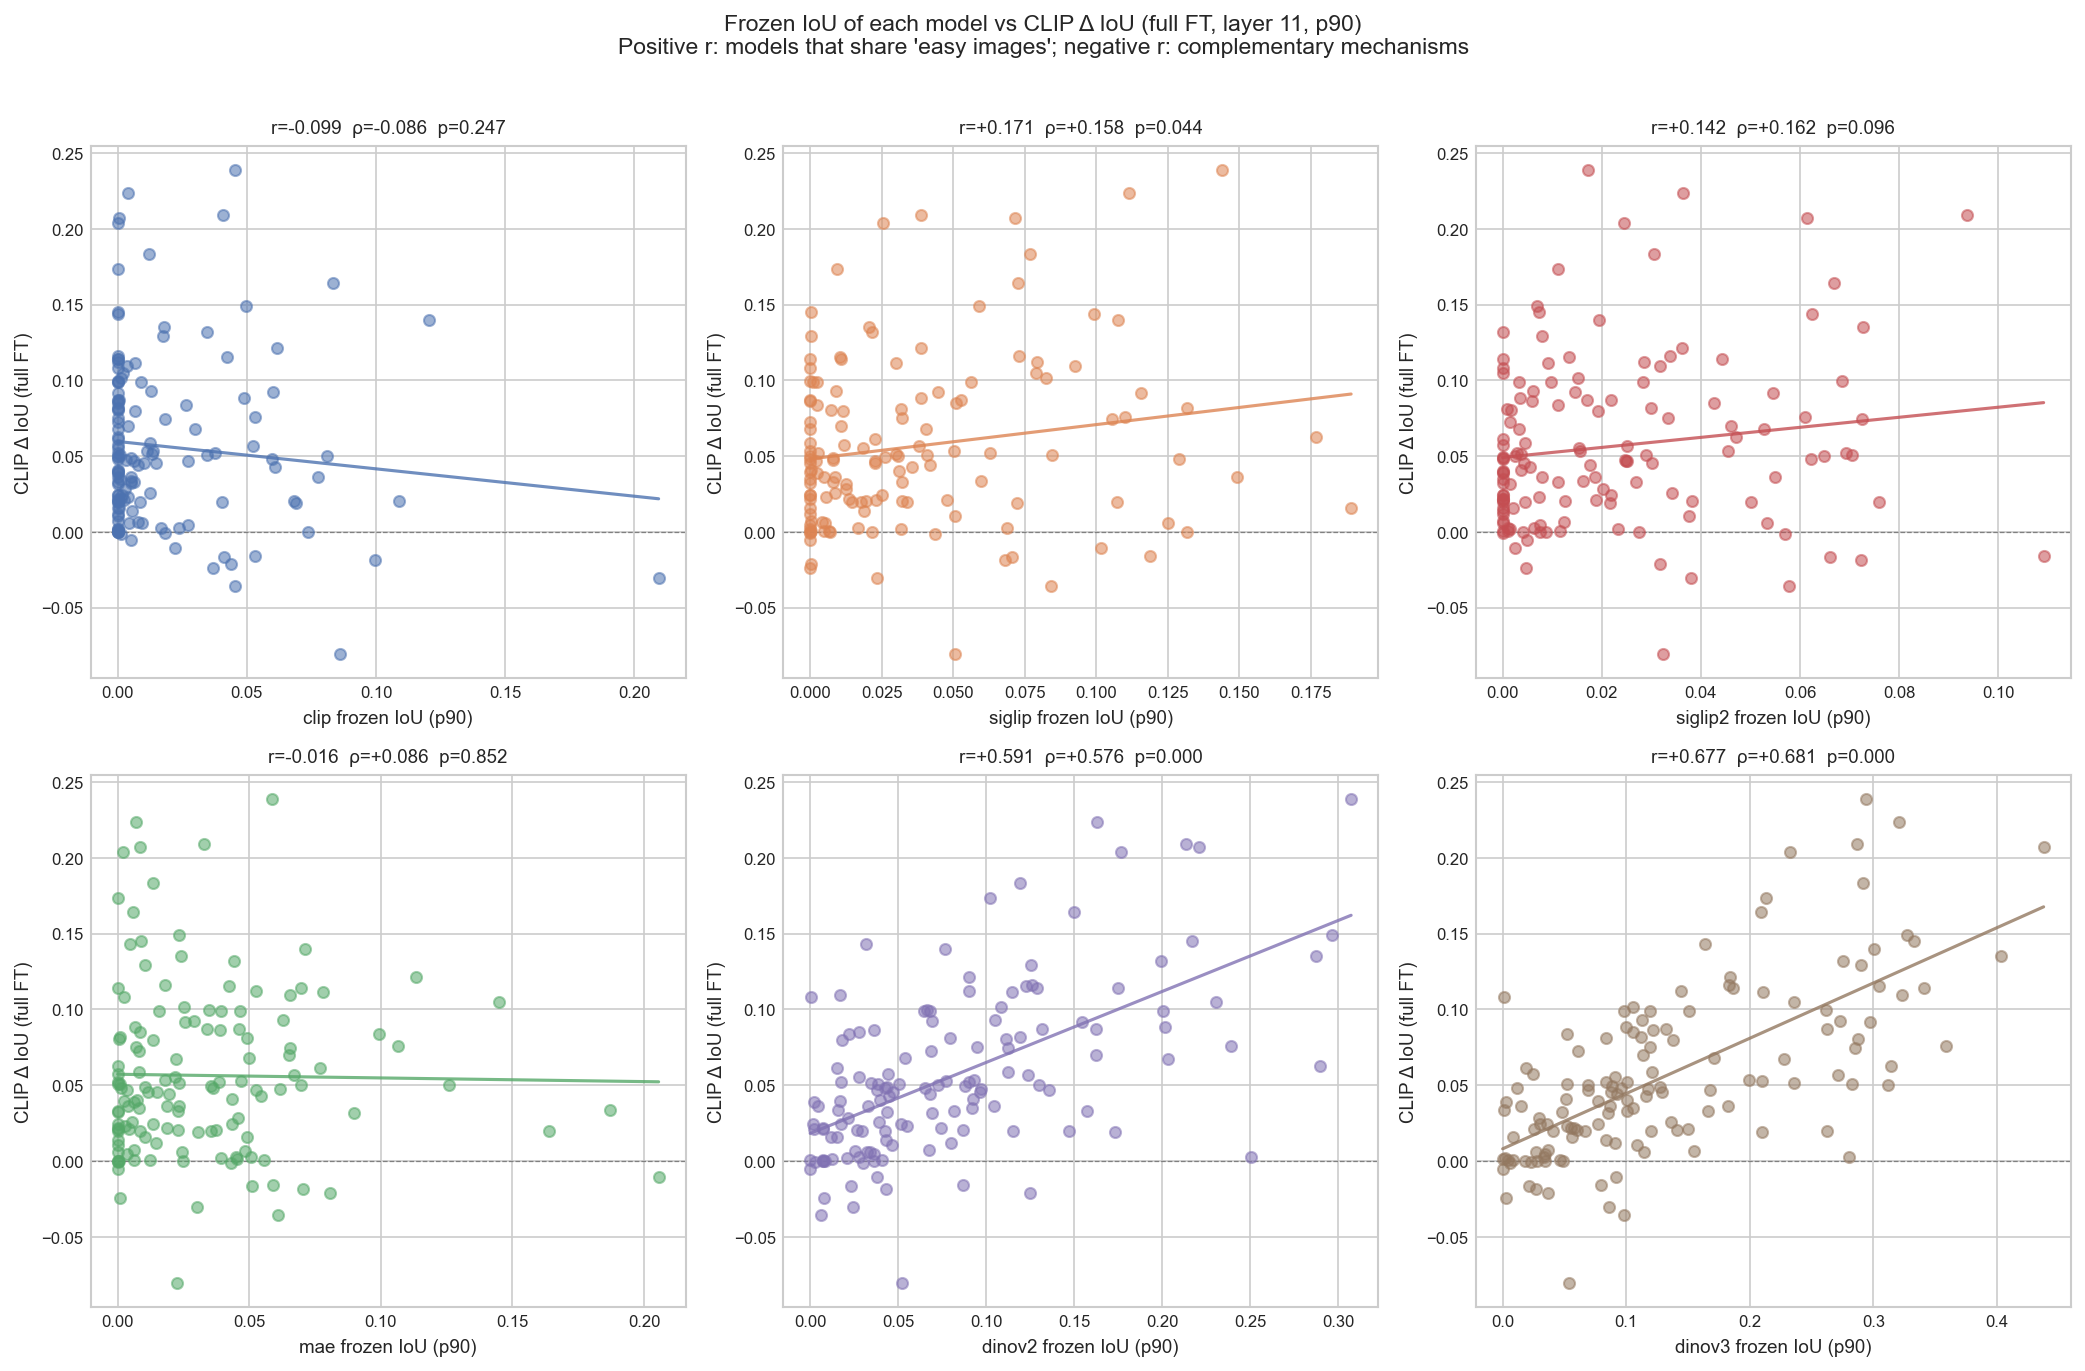
\includegraphics[width=\textwidth]{RQ3_model_correlation_scatter.png}
\caption{DINOv3 frozen IoU@90 vs.\ CLIP $\Delta$IoU@90 per image ($r\!=\!+0.677$). Structural image difficulty, not model family, determines what is ``easy''.}
\label{figure RQ3 model scatter}
\end{figure}

Expert-aligned attention concentrates in a small number of heads rather than spreading uniformly across the transformer (Figure~\ref{figure RQ3 head ranking}). DINOv3 is the cleanest case: the same \texttt{layer10/head8} remains best across Frozen, LoRA, and Full, appearing in the top three on more than 110 of 139 images in every condition. DINOv2 shows the same preserved-head pattern at lower absolute alignment. MAE shifts from \texttt{layer10/head5} to \texttt{layer11/head7} under LoRA, then returns to \texttt{layer10/head5} under Full. CLIP is the clearest reorganisation case: frozen CLIP's best heads sit in early layers (\texttt{layer4/head5} leads at mean IoU@90~$=$~0.067), while the selected late layer used in the delta view is weak before adaptation (\texttt{layer11} max IoU@90~$=$~0.034) and then becomes the strongest adapted layer (best \texttt{layer11} head reaches 0.084 under LoRA and 0.105 under Full), with \texttt{layer4/head5} staying near its frozen score. Coverage and EMD agree on the high-level reading, with DINO-family stability being cross-metric while MAE and CLIP preserve only the broader adaptation pattern rather than the exact winning head.

% \begin{figure}[!h]
% \centering
% 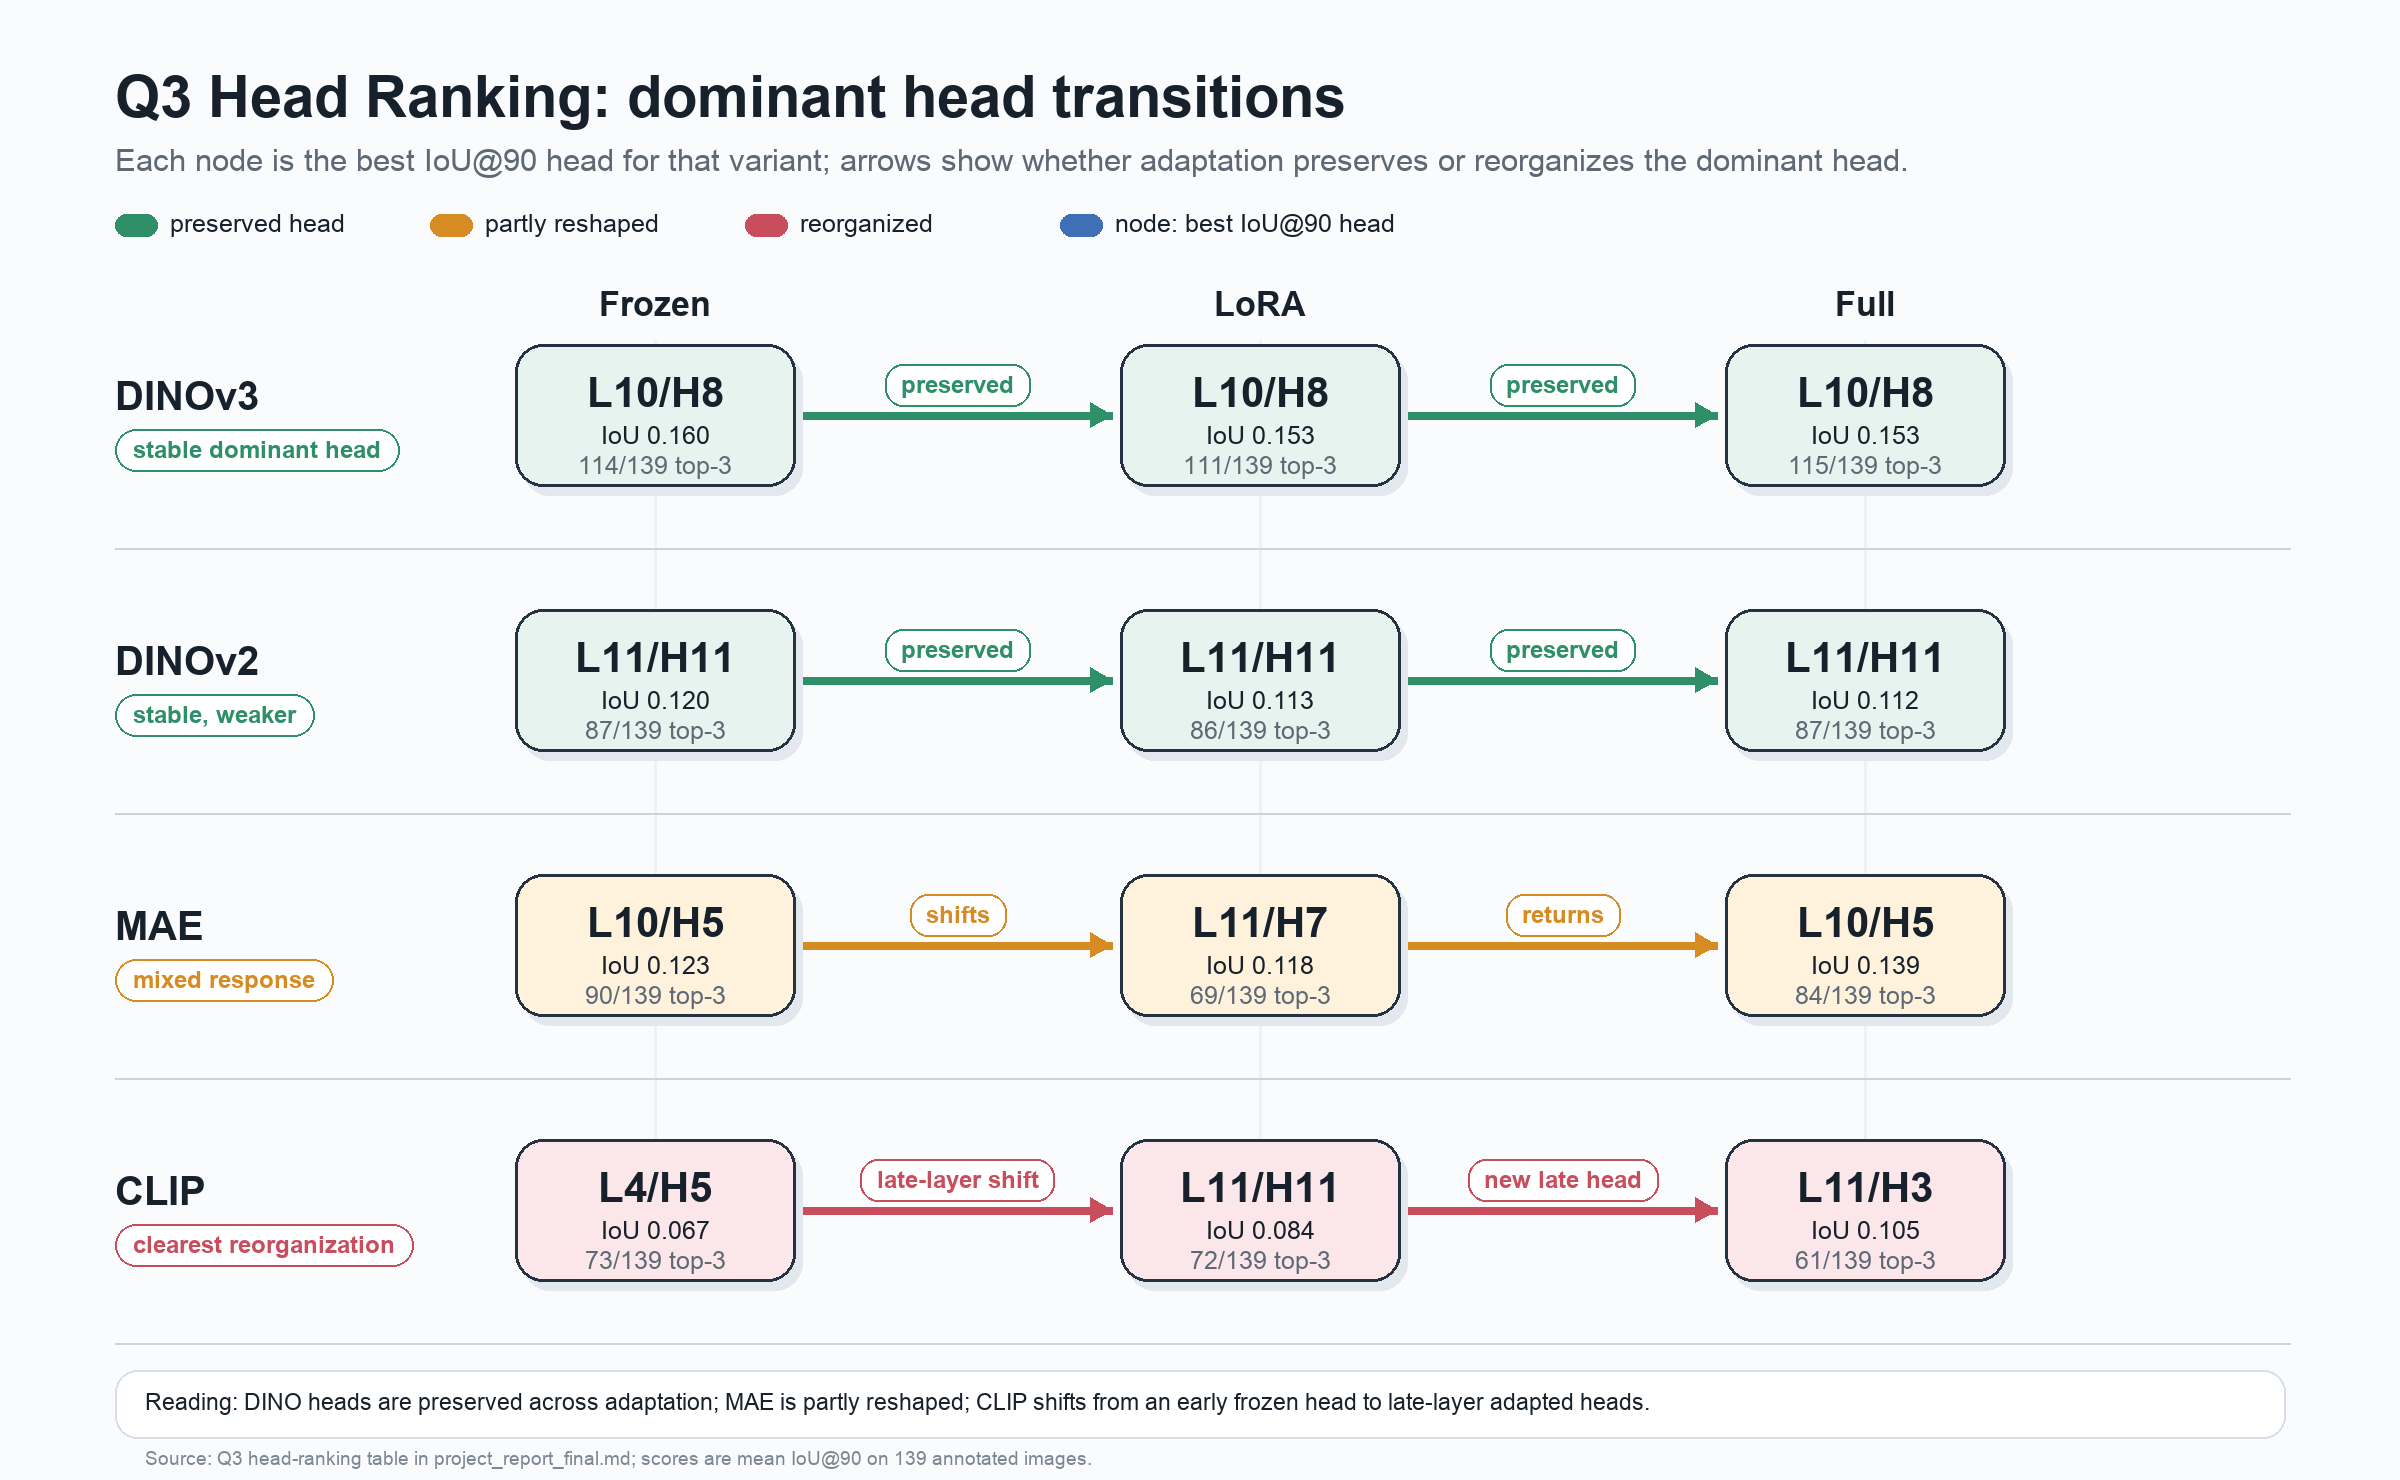
\includegraphics[width=\textwidth]{RQ3_head_ranking_transition_map.png}
% \caption{Q3 head-ranking transition map. Each node is the best IoU@90 head
% for a model variant, with mean IoU@90 and top-3 frequency across the 139
% annotated images. DINO-family models preserve their dominant heads across
% adaptation; MAE shows a mixed pattern; CLIP shifts from an early frozen head
% to late-layer adapted heads.}
% \label{figure RQ3 head ranking}
% \end{figure}


\begin{table}[!h]
\caption{Q3 head-ranking transition map. Each node is the best IoU@90 head for a model variant, with mean IoU@90 and top-3 frequency across the 139 annotated images. DINO-family models preserve their dominant heads across adaptation; MAE shows a mixed pattern; CLIP shifts from an early frozen head to late-layer adapted heads. \textcolor{red}{TJ: Shall we add SIgLIP, SIgLIP2 and linear probe?}\label{table RQ3 head ranking}}
\begin{tabular}{l|cccccc}
\hline
Vision & \multicolumn{6}{c}{Fine-tuning strategy}  \\
foundation & \multicolumn{2}{c}{Frozen} & \multicolumn{2}{c}{LoRA} & \multicolumn{2}{l}{Full fine-tuning} \\
model & Layer & Head & Layer & Head & Layer & Head \\ \hline
DINOv2 & 10 & 8 & 10 & 8 & 10 & 8 \\
DINOv3 & 11 & 11 & 11 & 11 & 11 & 11 \\
CLIP & 10 & 5 & 11 & 7 & 10 & 5 \\
MAE & 4 & 5 & 11 & 11 & 11 & 3 \\ \hline
\end{tabular}
\end{table}


% \begin{figure}[h]
%   \centering
%   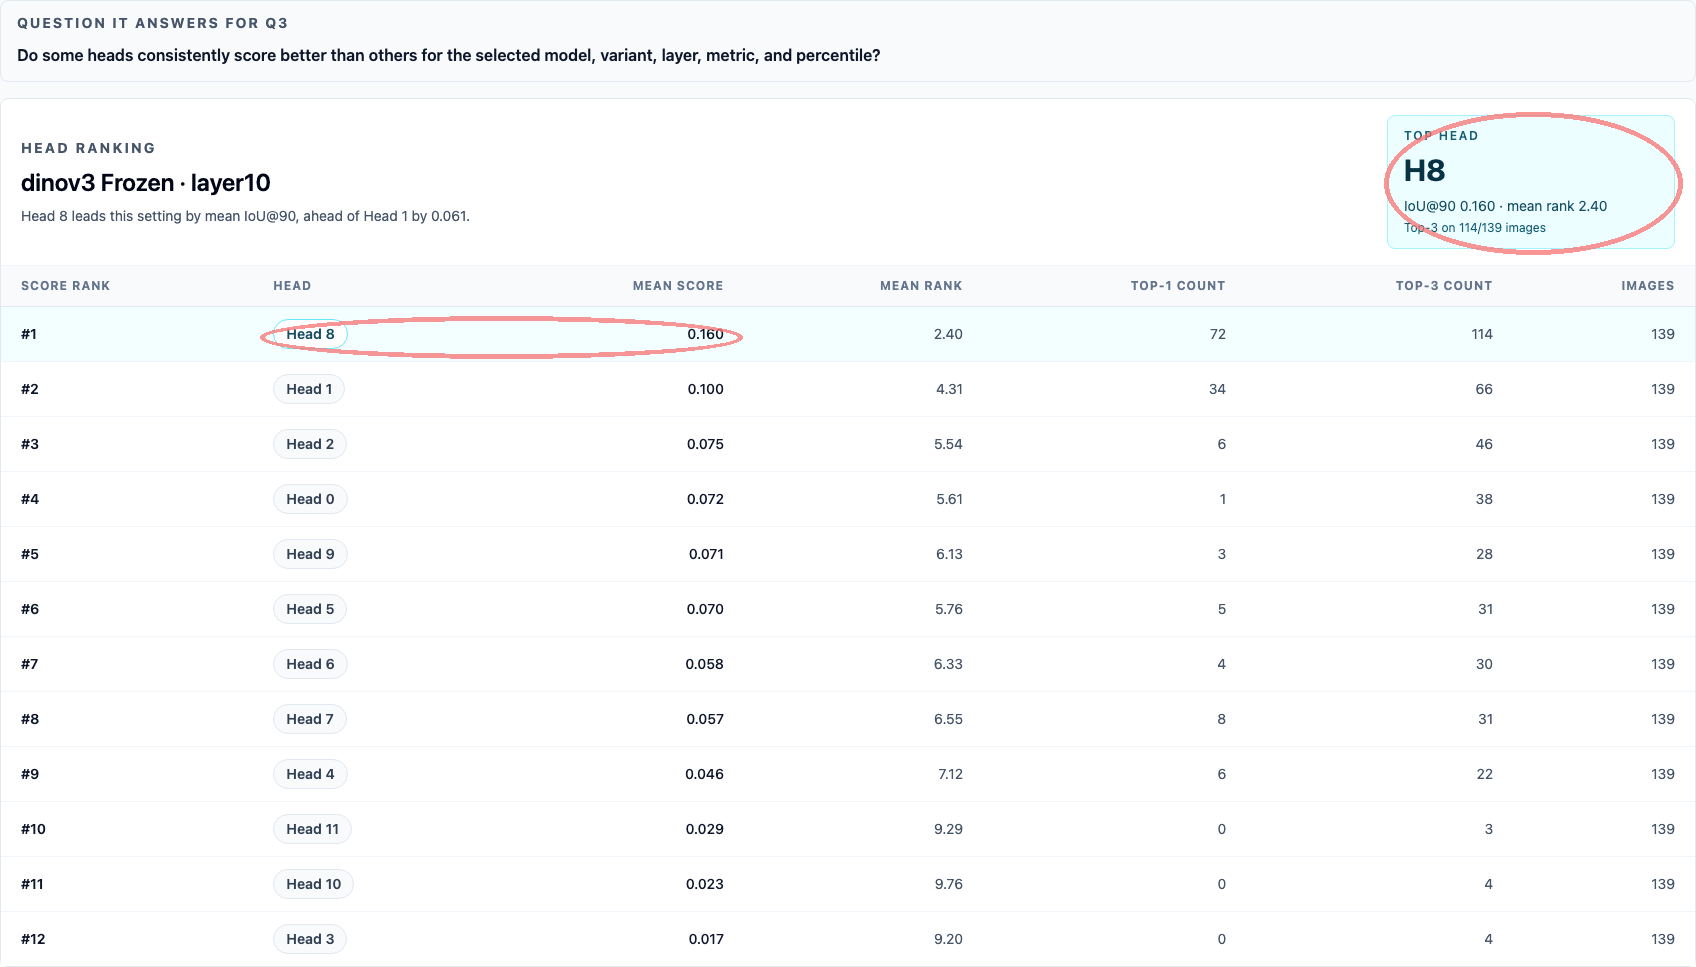
\includegraphics[width=\textwidth]{q3_head_ranking_report_view.png}
%   \caption{DINOv3 frozen head-ranking drill-down at \texttt{layer10} using
%   IoU@90. Head~8 leads with mean IoU@90~$=$~0.160, mean rank~2.40, and top-3
%   placement on 114/139 images, supporting the sparsity claim behind the
%   transition map.}
%   \label{fig:q3_ranking_dinov3}
% \end{figure}

The same concentration pattern holds across the full $12 \times 12$ grid of (layer, head) pairs. In each frozen scoped model, the top-ranked pair's mean IoU@90 lands $2.7\times$--$3.5\times$ above the median pair's (DINOv3 $3.45\times$, CLIP $3.22\times$, MAE $2.92\times$, DINOv2 $2.69\times$). The five best pairs together account for $7.3\%$--$9.0\%$ of total mean IoU@90 across all 144 pairs, roughly $2\times$ the $3.5\%$ they would hold if alignment were uniform. This is the quantitative content of ``sparse'': expert-aligned signal concentrates in a small minority of heads rather than spreading evenly. This connects to Q2. DINO-family models already have strong frozen spatial alignment, so fine-tuning mostly preserves the dominant expert-aligned head. CLIP and MAE gain more from adaptation, and RQ3 shows that those gains can come from \emph{different heads} becoming best aligned after fine-tuning. CLIP's \texttt{layer11} alignment is newly strengthened by adaptation rather than inherited from an already strong frozen \texttt{layer11} head, while MAE is selectively reshaped toward discriminative geometric forms.


\subsection{Discussion}

\textbf{Intuitive findings.} Linear Probe as a true attention-change control validates that RQ2 movement reflects representation change, not a reporting artefact. Stronger task-conditioned adaptation helps most when the frozen model is not yet strongly aligned - CLIP, MAE, and SigLIP-family results fit this pattern.

\textbf{Surprising findings.} The SigLIP family pairs excellent frozen MSE with EMD worse than random, illustrating why single-metric interpretation is dangerous. DINOv2 does not improve dramatically under RQ2 despite other families gaining substantially: self-distillation may already produce more part-like spatial attention, leaving less headroom for downstream adaptation.

\textbf{Pretraining objective account.} CLIP's InfoNCE loss~\cite{Radford21CLIP} applies no patch-level spatial pressure; fine-tuning is the first spatial signal, and the gain concentrates on styles whose features are linguistically described. MAE's 75\%-masking objective~\cite{He22MAE} forces precise local geometry representations, which explains its Renaissance pediment affinity. DINOv3's Gram-anchoring loss~\cite{Simeoni26DINOv3} explicitly preserves second-order spatial structure, explaining its $\Delta\!\approx\!0$ result under Q2.

\textbf{Practical implications.} Model selection for domain adaptation should not be guided by accuracy alone. DINOv3 may be preferable when plausible evidence use matters without adaptation; CLIP or MAE become more attractive when adaptation is allowed. LoRA captures most of the attention-shift benefit in several models with fewer regressions than Full fine-tuning. MAE is the only model whose per-image $\Delta$ is anti-correlated with the language cluster, making it the natural complementary partner in coverage-seeking ensembles.

\subsection{Limitations}

The annotated evaluation subset is small (139 images), limiting statistical power. Bounding boxes are expert-guided but not exhaustive, introducing sparse annotation bias, especially for Baroque. Attention is an incomplete explanation signal: strong alignment is evidence of plausibility, not causal proof. IoU depends on the thresholding rule; continuous metrics require calibration to avoid overreading raw numbers.

\section{Conclusions} \label{section conclusions}

This paper asks whether self-supervised vision foundation models attend to the same architectural evidence that experts consider diagnostically important. Using WikiChurches, expert bounding boxes, and a multi-metric alignment framework, we address three linked questions across seven models and three fine-tuning strategies.

For \textbf{Q1}, frozen expert-aligned attention exists but is not evenly distributed. DINOv3 provides the strongest evidence, leading the default-method benchmark on IoU, Coverage, KL, and EMD and clearing all calibrated baselines. Base SigLIP is a stronger frozen overlap result than SigLIP2 at its best mean-attention layer, but both variants still have late-layer adaptation headroom. The safest interpretation is not that all SSL models attend like experts, but that DINOv3's spatial prior is unusually compatible with expert-marked architectural evidence in WikiChurches.

For \textbf{Q2}, per-head specialisation is sparse, descriptive, and family-shaped. DINOv3's \texttt{layer10/head8} and DINOv2's \texttt{layer11/head11} remain dominant across Frozen, LoRA, and Full, consistent with the DINO family's already-strong spatial prior. MAE is partly reshaped by adaptation, while CLIP shows the clearest reorganisation from an earlier frozen head to later adapted heads. The strongest head-linked architectural features cluster on portals, arches, and rose-window-scale structures, so the safest claim is not that heads are exact architectural-part detectors, but that some heads expose spatial patterns more compatible with expert-marked structure than others.

For \textbf{Q3}, fine-tuning's effect is mediated by three interacting factors: the pretraining objective's spatial prior (DINO preserves strong frozen alignment; CLIP, MAE, and SigLIP-family gain because they lack it); dataset linguistic coverage (CLIP's gain concentrates on Gothic and Romanesque features densely described in English web text); and geometric discriminability (MAE redirects attention to Renaissance-exclusive pediment forms that pixel reconstruction already encodes with high local fidelity). Models with different objectives converge on the same structurally easy images rather than complementary subsets, with implications for ensembling strategies.






\cite{*}

\backmatter


\section*{Declarations}

\textbf{Funding}

This research received no external funding. \newline

\noindent\textbf{Competing interests}

The authors declare no financial or commercial conflicts of interest. \newline

\noindent\textbf{Ethics approval and consent to participate}

Not applicable.\newline

\noindent\textbf{Consent for publication}

Not applicable.\newline

\noindent\textbf{Data availability }

The dataset that supports the findings of this study is provided in \cite{Barz21WikiChurches}. \newline

\noindent\textbf{Code availability }

The code that supports the findings of this study is available on the GitHub repository \url{https://github.com/XXX}.\newline

\noindent\textbf{Author contribution}

% Please choose from the following list. It is okay for multiple authors to choose the same items. No need to cover the entire list because some items are not applicable.

First author: 

Second author:

J. Tian: Formal analysis, Writing - Original Draft, Writing - Review \& Editing, Supervision.

X. Xie: Formal analysis, Writing - Original Draft, Writing - Review \& Editing.

% Choose from the following list, 
% % https://www.elsevier.com/researcher/author/policies-and-guidelines/credit-author-statement
% Conceptualization
% Methodology
% Software
% Validation
% Formal analysis
% Investigation
% Resources
% Data Curation
% Writing - Original Draft
% Writing - Review \& Editing
% Visualization
% Supervision
% Project administration
% Funding acquisition

%%===========================================================================================%%
%% If you are submitting to one of the Nature Portfolio journals, using the eJP submission   %%
%% system, please include the references within the manuscript file itself. You may do this  %%
%% by copying the reference list from your .bbl file, paste it into the main manuscript .tex %%
%% file, and delete the associated \verb+\bibliography+ commands.                            %%
%%===========================================================================================%%

\bibliography{xvision}% common bib file


\end{document}
